\chapter{Results}
\label{ch:evaluation}

This chapter reports cohort characteristics, sample-size adequacy, model
performance and calibration, clinical utility, external validation,
label-anchor analyses, the feature ablation, model diagnostics, equity analyses
and, last, the variance decomposition and pre-registered hypothesis verdicts
(Section~\ref{sec:decomposition}), which are assembled from the earlier
estimates. Results are marked as confirmatory [C], exploratory [E] or
descriptive [D] (Section~\ref{sec:inference}); the status of every analysis is
recorded in the analysis register (Appendix~\ref{sec:register}). Unless
otherwise stated, intervals are 95\% stay-level cluster-bootstrap intervals.
Chapter~\ref{ch:discussion} interprets the results and sets out the
limitations.

%===========================================================================


\section{Cohort Description and Label Variation \texorpdfstring{[D]}{[D]}}
\label{sec:cohort_results}
%===========================================================================

Table~\ref{tab:cohort} summarises the three cohorts. The base extraction
identifies \pcNStays{} adult first ICU stays. The database and patients are the
same across all three variants; only the sepsis definition differs.

\begin{table}[H]
    \centering\small
    \adjustbox{max width=\textwidth}{%
    \begin{tabular}{llrrrrr}
        \toprule
        \textbf{Var} & \textbf{Name} & \textbf{Stays} & \textbf{Onsets (cohort)}
        & \textbf{\%} & \textbf{Deaths, no sepsis} & \textbf{Onset h (IQR)} \\
        \midrule
        A & Narrow      & \pcNStays & \pcNOnsetsA & \pcPctOnsetsA & \pcNDeathsNoSepA & \pcMedianOnsetHA [\pcIqrOnsetLoHA--\pcIqrOnsetHiHA] \\
        B & Seymour-Std & \pcNStays & \pcNOnsetsB & \pcPctOnsetsB & \pcNDeathsNoSepB & \pcMedianOnsetHB [\pcIqrOnsetLoHB--\pcIqrOnsetHiHB] \\
        C & Liberal     & \pcNStays & \pcNOnsetsC & \pcPctOnsetsC & \pcNDeathsNoSepC & \pcMedianOnsetHC [\pcIqrOnsetLoHC--\pcIqrOnsetHiHC] \\
        \bottomrule
    \end{tabular}}
    \caption{Cohort description by label variant. ``Deaths, no sepsis'' counts
    stays ending in death with no labelled sepsis onset before it, so it varies
    with the label. The Liberal variant's wider antibiotic-culture windows and
    rolling SOFA baseline identify about twice as many cases. Onsets are counted
    \textbf{cohort-wide, at any hour of the stay}; the subset inside the 72-hour
    modelling horizon (\pcNPositiveA, \pcNPositiveBPanel{} and \pcNPositiveC),
    on which the models are trained and evaluated, is reported in
    Table~\ref{tab:label_agreement}.}
    \label{tab:cohort}
\end{table}

The twofold difference in sepsis prevalence between Variant A
(\pcPctOnsetsA\%) and Variant C (\pcPctOnsetsC\%) is consistent with the label
sensitivity previously reported by Johnson et al.\ \cite{johnson2018comparative}.

%===========================================================================


\section{Sample Size Adequacy \texorpdfstring{[C]}{[C]}}
\label{sec:sample_size_results}
%===========================================================================

Because Riley et al.'s criteria \cite{riley2019sample} assume independent
observations, adequacy is assessed on the stay rather than the person-hour
(Section~\ref{sec:sample_size}; Table~\ref{tab:sample_size}).

\begin{table}[H]
    \centering\small
    \begin{tabular}{llrrrrr}
        \toprule
        \textbf{Var} & \textbf{Name} & \textbf{Train}
        & \textbf{Sepsis} & \textbf{Stay}
        & \textbf{Riley min-$N$} & \textbf{EPV} \\
        & & \textbf{stays} & \textbf{stays} & \textbf{prev.}
        & \textbf{(stays)} & \\
        \midrule
        A & Narrow      & \pcNTrainStays & \pcNOnsetEventsA & \pcStayPrevalenceA & \pcMinNRileyStayA & \pcEpvA \\
        B & Seymour-Std & \pcNTrainStays & \pcNOnsetEventsB & \pcStayPrevalenceB & \pcMinNRileyStayB & \pcEpvB \\
        C & Liberal     & \pcNTrainStays & \pcNOnsetEventsC & \pcStayPrevalenceC & \pcMinNRileyStayC & \pcEpvC \\
        \bottomrule
    \end{tabular}
    \caption{Sample size adequacy on the independent unit. Every row is a count
    of \emph{stays}: the training split contains \pcNTrainStays{} stays, of
    which the given number are labelled septic under that variant. Riley
    min-$N$ is the minimum number of independent observations required at that
    variant's stay-level prevalence, an anticipated $C$-statistic of
    \pcAnticipatedAuc{} \cite{moor2023review}, and
    \pcNCandidatePredictors{} parameters, which is the number of terms in the
    sepsis-specific linear predictor (\pcHTwoNTerms{} covariates, a six-column
    spline baseline and an intercept). The criterion is applied as an
    approximate binary-outcome assessment of the sepsis-versus-at-risk contrast
    (Section~\ref{sec:sample_size}); EPV is events per parameter on that
    reading. All three variants exceed the requirement by a wide margin
    (\pcRileyMarginA$\times$, \pcRileyMarginB$\times$ and
    \pcRileyMarginC$\times$ respectively).}
    \label{tab:sample_size}
\end{table}

The corresponding design matrices contain \pcNTrainPersonHA{},
\pcNTrainPersonHB{} and \pcNTrainPersonHC{} training person-hours, at per-hour
event rates of \pcPerHourRateA{}, \pcPerHourRateB{} and \pcPerHourRateC{}.
These figures govern the computational cost of the fit but do not multiply the
effective sample size.

Sample size is therefore not a binding constraint: under the primary label the
requirement is \pcMinNRileyStayB{} independent observations against
\pcNTrainStays{} available, a margin of \pcRileyMarginB$\times$. Precision is
limited instead in the external cohort
(Section~\ref{sec:external_interpretability}) and in the smaller demographic
strata (Section~\ref{sec:equity}).

%===========================================================================


\section{Model Performance: Internal Temporal Evaluation \texorpdfstring{[C]}{[C]}}
\label{sec:internal_performance}
%===========================================================================

Table~\ref{tab:internal_results} reports performance on the temporal test set
(2017--2019) under the unrestricted evaluation window.

\begin{table}[H]
    \centering\small
    \begin{tabular}{llrrrrr}
        \toprule
        \textbf{Var} & \textbf{Model}
        & \textbf{AUROC} & \textbf{AUPRC}
        & \textbf{Utility} & \textbf{Utility} & \textbf{Alert} \\
        & & & & \textbf{(0.5)} & \textbf{(best)} & \textbf{burden} \\
        \midrule
        A & Primary & \pcAurocPrimaryA & \pcAuprcPrimaryA & \pcUtilityPrimaryA & \pcUtilityMaxPrimaryA & \pcAlertBurdenPrimaryA \\
        A & GBT     & \pcAurocGbtA     & \pcAuprcGbtA     & \pcUtilityGbtA     & \pcUtilityMaxGbtA     & \pcAlertBurdenGbtA     \\
        A & NEWS2   & \pcAurocNewsA    & \pcAuprcNewsA    & \pcUtilityNewsA    & \pcUtilityMaxNewsA    & \pcAlertBurdenNewsA    \\
        A & Cox     & \pcAurocCoxA     & \pcAuprcCoxA     & \pcUtilityCoxA     & \pcUtilityMaxCoxA     & \pcAlertBurdenCoxA     \\
        A & qSOFA   & \pcAurocQsofaA   & \pcAuprcQsofaA   & \pcUtilityQsofaA   & \pcUtilityMaxQsofaA   & \pcAlertBurdenQsofaA   \\
        A & SIRS    & \pcAurocSirsA    & \pcAuprcSirsA    & \pcUtilitySirsA    & \pcUtilityMaxSirsA    & \pcAlertBurdenSirsA    \\
        \midrule
        B & Primary & \pcAurocPrimaryB & \pcAuprcPrimaryB & \pcUtilityPrimaryB & \pcUtilityMaxPrimaryB & \pcAlertBurdenPrimaryB \\
        B & GBT     & \pcAurocGbtB     & \pcAuprcGbtB     & \pcUtilityGbtB     & \pcUtilityMaxGbtB     & \pcAlertBurdenGbtB     \\
        B & NEWS2   & \pcAurocNewsB    & \pcAuprcNewsB    & \pcUtilityNewsB    & \pcUtilityMaxNewsB    & \pcAlertBurdenNewsB    \\
        B & Cox     & \pcAurocCoxB     & \pcAuprcCoxB     & \pcUtilityCoxB     & \pcUtilityMaxCoxB     & \pcAlertBurdenCoxB     \\
        B & qSOFA   & \pcAurocQsofaB   & \pcAuprcQsofaB   & \pcUtilityQsofaB   & \pcUtilityMaxQsofaB   & \pcAlertBurdenQsofaB   \\
        B & SIRS    & \pcAurocSirsB    & \pcAuprcSirsB    & \pcUtilitySirsB    & \pcUtilityMaxSirsB    & \pcAlertBurdenSirsB    \\
        \midrule
        C & Primary & \pcAurocPrimaryC & \pcAuprcPrimaryC & \pcUtilityPrimaryC & \pcUtilityMaxPrimaryC & \pcAlertBurdenPrimaryC \\
        C & GBT     & \pcAurocGbtC     & \pcAuprcGbtC     & \pcUtilityGbtC     & \pcUtilityMaxGbtC     & \pcAlertBurdenGbtC     \\
        C & NEWS2   & \pcAurocNewsC    & \pcAuprcNewsC    & \pcUtilityNewsC    & \pcUtilityMaxNewsC    & \pcAlertBurdenNewsC    \\
        C & Cox     & \pcAurocCoxC     & \pcAuprcCoxC     & \pcUtilityCoxC     & \pcUtilityMaxCoxC     & \pcAlertBurdenCoxC     \\
        C & qSOFA   & \pcAurocQsofaC   & \pcAuprcQsofaC   & \pcUtilityQsofaC   & \pcUtilityMaxQsofaC   & \pcAlertBurdenQsofaC   \\
        C & SIRS    & \pcAurocSirsC    & \pcAuprcSirsC    & \pcUtilitySirsC    & \pcUtilityMaxSirsC    & \pcAlertBurdenSirsC    \\
        \bottomrule
    \end{tabular}
    \caption{Internal temporal test performance (2017--2019, all variants use
    temporal split). N test rows: \pcNTestRowsB{} (B). \textbf{Utility (0.5)} is
    the normalised adapted PhysioNet-style Utility Score
    (Section~\ref{sec:metrics}) at the default cut-off;
    \textbf{Utility (best)} is its maximum over the threshold grid of
    Section~\ref{sec:metrics}. Zero is the no-alert strategy under both. Alert
    burden is at the 0.5 cut-off ($\infty$ = no true alerts there); the
    benchmark is 1.4 \cite{moor2023review}. Per-threshold curves are in
    Figure~\ref{fig:utility_sweep} and the attaining operating points in
    Table~\ref{tab:utility_optimum}. Confidence intervals for Variant B are in
    Table~\ref{tab:internal_ci}. \textbf{[C] confirmatory.}}
    \label{tab:internal_results}
\end{table}

\begin{table}[H]
    \centering\small
    \begin{tabular}{llll}
        \toprule
        \textbf{Model} & \textbf{AUROC} & \textbf{95\% CI} & \textbf{AUPRC (95\% CI)} \\
        \midrule
        Primary & \pcAurocPrimaryB & \pcAurocCiLoPrimaryB--\pcAurocCiHiPrimaryB & \pcAuprcPrimaryB{} \pcAuprcCiPrimaryB \\
        GBT     & \pcAurocGbtB     & \pcAurocCiLoGbtB--\pcAurocCiHiGbtB         & \pcAuprcGbtB{} \pcAuprcCiGbtB     \\
        NEWS2   & \pcAurocNewsB    & \pcAurocCiLoNewsB--\pcAurocCiHiNewsB       & \pcAuprcNewsB{} \pcAuprcCiNewsB    \\
        Cox     & \pcAurocCoxB     & \pcAurocCiLoCoxB--\pcAurocCiHiCoxB         & \pcAuprcCoxB{} \pcAuprcCiCoxB     \\
        qSOFA   & \pcAurocQsofaB   & \pcAurocCiLoQsofaB--\pcAurocCiHiQsofaB     & \pcAuprcQsofaB{} \pcAuprcCiQsofaB   \\
        SIRS    & \pcAurocSirsB    & \pcAurocCiLoSirsB--\pcAurocCiHiSirsB       & \pcAuprcSirsB{} \pcAuprcCiSirsB    \\
        \bottomrule
    \end{tabular}
    \caption{Variant B temporal test performance with 95\% stay-level
    cluster-bootstrap intervals ($B = 2{,}000$ replicates over
    \pcNTestRowsB{} test person-hours carrying \pcNTestEventsB{} sepsis onsets).
    These are \emph{marginal} intervals; paired differences are reported
    separately where claimed (H6, Section~\ref{sec:h6}). The primary model and
    GBT overlap almost completely, and both are separated from the other four
    models. \textbf{[C] confirmatory.}}
    \label{tab:internal_ci}
\end{table}

\subsection{Utility and Alert Burden Across Thresholds}
\label{sec:utility_threshold}

At the default 0.5 cut-off no model does better than issuing no alerts, but
this threshold is uninformative. The primary model scores \pcUtilityPrimaryB{}
under Variant B because its largest predicted hourly probability is far below
0.5, so it generates no alert. The models that do cross 0.5 (the rule-based
scores, rescaled onto the unit interval, and the Cox linear predictor) do so
so often that they score well below zero: \pcUtilityCoxB{} for Cox and
\pcUtilityQsofaB{} for qSOFA under Variant B. At this cut-off the models are
therefore separated by calibration rather than clinical value.

\begin{figure}[H]
    \centering
    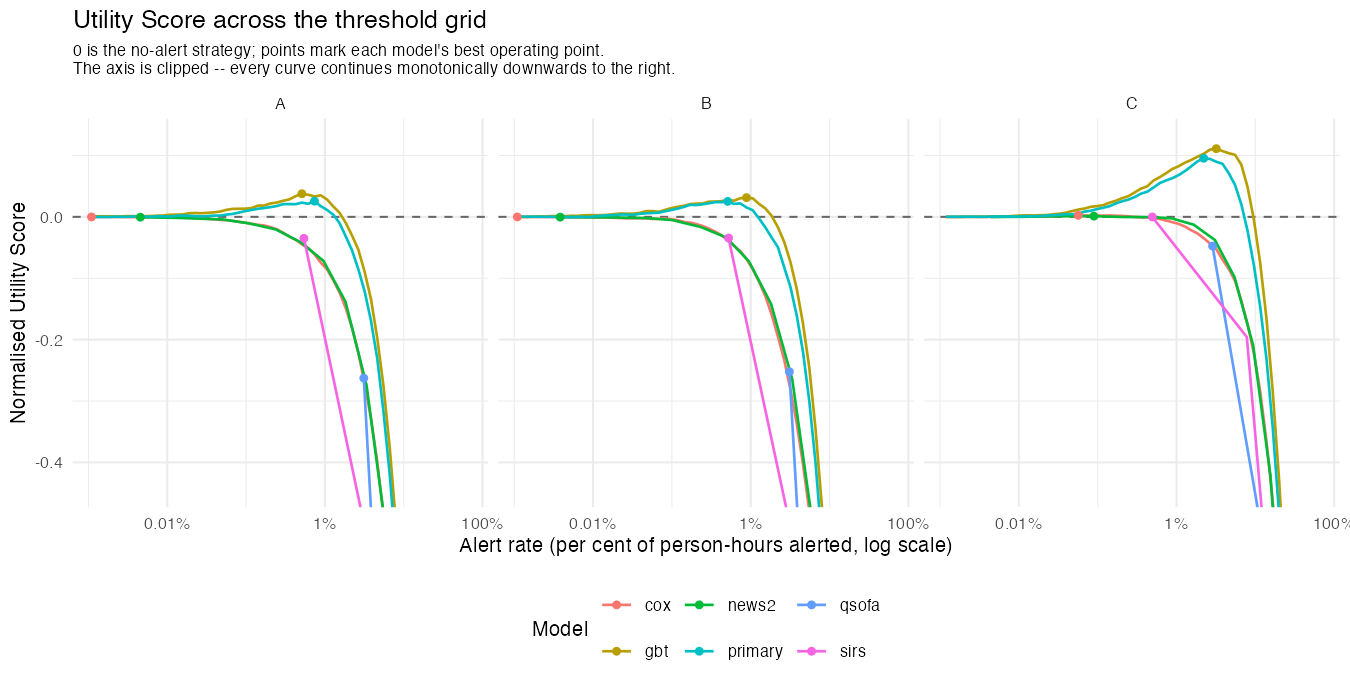
\includegraphics[width=\textwidth]{images/07_utility_threshold_sweep.png}
    \caption{Normalised Utility Score against alert rate for every model and
    pre-registered label variant on the temporal test set. The dashed line at
    zero is the no-alert strategy, and points mark each model's best operating
    point. Only the primary model and GBT rise above zero, peaking between 0.5
    and 3 per cent of person-hours alerted. The vertical axis is clipped; every
    curve falls to $-5$ or below at a 50 per cent alert rate.}
    \label{fig:utility_sweep}
\end{figure}

Figure~\ref{fig:utility_sweep} traces the whole threshold grid, and
Table~\ref{tab:utility_optimum} reports each model's best attainable score
together with the operating point that attains it.

\begin{table}[H]
    \centering\small
    \begin{tabular}{llrrrr}
        \toprule
        \textbf{Var} & \textbf{Model} & \textbf{Max utility}
        & \textbf{Alert rate} & \textbf{Stays} & \textbf{Alert} \\
        & & & \textbf{(\% p-h)} & \textbf{detected (\%)} & \textbf{burden} \\
        \midrule
        A & Primary & \pcUtilityMaxPrimaryA & \pcUtilityOptAlertPctPrimaryA & \pcUtilityOptDetectPctPrimaryA & \pcUtilityOptBurdenPrimaryA \\
        A & GBT     & \pcUtilityMaxGbtA     & \pcUtilityOptAlertPctGbtA     & \pcUtilityOptDetectPctGbtA     & \pcUtilityOptBurdenGbtA     \\
        A & NEWS2   & \pcUtilityMaxNewsA    & \pcUtilityOptAlertPctNewsA    & \pcUtilityOptDetectPctNewsA    & \pcUtilityOptBurdenNewsA    \\
        A & Cox     & \pcUtilityMaxCoxA     & \pcUtilityOptAlertPctCoxA     & \pcUtilityOptDetectPctCoxA     & \pcUtilityOptBurdenCoxA     \\
        A & qSOFA   & \pcUtilityMaxQsofaA   & \pcUtilityOptAlertPctQsofaA   & \pcUtilityOptDetectPctQsofaA   & \pcUtilityOptBurdenQsofaA   \\
        A & SIRS    & \pcUtilityMaxSirsA    & \pcUtilityOptAlertPctSirsA    & \pcUtilityOptDetectPctSirsA    & \pcUtilityOptBurdenSirsA    \\
        \midrule
        B & Primary & \pcUtilityMaxPrimaryB & \pcUtilityOptAlertPctPrimaryB & \pcUtilityOptDetectPctPrimaryB & \pcUtilityOptBurdenPrimaryB \\
        B & GBT     & \pcUtilityMaxGbtB     & \pcUtilityOptAlertPctGbtB     & \pcUtilityOptDetectPctGbtB     & \pcUtilityOptBurdenGbtB     \\
        B & NEWS2   & \pcUtilityMaxNewsB    & \pcUtilityOptAlertPctNewsB    & \pcUtilityOptDetectPctNewsB    & \pcUtilityOptBurdenNewsB    \\
        B & Cox     & \pcUtilityMaxCoxB     & \pcUtilityOptAlertPctCoxB     & \pcUtilityOptDetectPctCoxB     & \pcUtilityOptBurdenCoxB     \\
        B & qSOFA   & \pcUtilityMaxQsofaB   & \pcUtilityOptAlertPctQsofaB   & \pcUtilityOptDetectPctQsofaB   & \pcUtilityOptBurdenQsofaB   \\
        B & SIRS    & \pcUtilityMaxSirsB    & \pcUtilityOptAlertPctSirsB    & \pcUtilityOptDetectPctSirsB    & \pcUtilityOptBurdenSirsB    \\
        \midrule
        C & Primary & \pcUtilityMaxPrimaryC & \pcUtilityOptAlertPctPrimaryC & \pcUtilityOptDetectPctPrimaryC & \pcUtilityOptBurdenPrimaryC \\
        C & GBT     & \pcUtilityMaxGbtC     & \pcUtilityOptAlertPctGbtC     & \pcUtilityOptDetectPctGbtC     & \pcUtilityOptBurdenGbtC     \\
        C & NEWS2   & \pcUtilityMaxNewsC    & \pcUtilityOptAlertPctNewsC    & \pcUtilityOptDetectPctNewsC    & \pcUtilityOptBurdenNewsC    \\
        C & Cox     & \pcUtilityMaxCoxC     & \pcUtilityOptAlertPctCoxC     & \pcUtilityOptDetectPctCoxC     & \pcUtilityOptBurdenCoxC     \\
        C & qSOFA   & \pcUtilityMaxQsofaC   & \pcUtilityOptAlertPctQsofaC   & \pcUtilityOptDetectPctQsofaC   & \pcUtilityOptBurdenQsofaC   \\
        C & SIRS    & \pcUtilityMaxSirsC    & \pcUtilityOptAlertPctSirsC    & \pcUtilityOptDetectPctSirsC    & \pcUtilityOptBurdenSirsC    \\
        \bottomrule
    \end{tabular}
    \caption{Maximum achievable Utility Score and the operating point that
    attains it, over the sixty-point threshold grid, on the temporal test set.
    ``Alert rate'' is the percentage of test person-hours alerted; ``stays
    detected'' is the percentage of septic stays alerted within the reward
    window $[\text{onset}-6,\ \text{onset}]$; alert burden is false alerts per
    true alert at that same point, against the benchmark of 1.4
    \cite{moor2023review}; $\infty$ with a maximum at or below zero means the
    best strategy is to raise no alert. \textbf{[E] exploratory:} thresholds
    are chosen on the test set, so these are upper bounds on achievable
    utility.}
    \label{tab:utility_optimum}
\end{table}

After threshold sweeping, the two fitted models reach positive utility under
every variant. Under Variant B their maximum scores
are \pcUtilityMaxPrimaryB{} (primary) and \pcUtilityMaxGbtB{} (GBT), on a
scale bounded above by 1. These optima are attained at
\pcUtilityOptBurdenPrimaryB{} and \pcUtilityOptBurdenGbtB{} false alerts per
true alert, while detecting \pcUtilityOptDetectPctPrimaryB{} and
\pcUtilityOptDetectPctGbtB{} per cent of septic stays within the actionable
window. Under Variants A and B, NEWS2, Cox, qSOFA and SIRS have no threshold at
which alerting beats not alerting, and under Variant C their maxima do not
exceed \pcUtilityMaxCoxC. Across all variants, every positive maximum
is attained at between \pcUtilityOptBurdenPrimaryC{} and
\pcUtilityOptBurdenGbtB{} false alerts per true alert, twenty to thirty-seven
times the benchmark of 1.4 \cite{moor2023review}. The thresholds are selected
on the test set, so these values are optimistic upper bounds. AUROC values in
the mid-to-high 0.7s (Table~\ref{tab:internal_results}) therefore did not
translate into an operating point with a clinically plausible alert burden.

Decision-curve net benefit prices false alarms differently: at a threshold
matched to the event prevalence, the primary model achieves positive net
benefit over both default strategies (Table~\ref{tab:net_benefit},
Section~\ref{sec:clinical_utility}). This is an internal contrast between two
metrics, not a test of H5's internal-to-external estimand. Under both metrics,
no configuration tested approaches the alert-burden benchmark.

\subsection{Calibration \texorpdfstring{[C]}{[C]}}
\label{sec:calibration_results}

Calibration intercept and slope are two summary numbers describing a whole
curve, so both the curve itself and a scalar summary of its distance from the
diagonal are reported. Following Van Calster et al.\
\cite{vancalster2019calibration}, the flexible calibration curve is a
restricted cubic spline of the outcome on the logit of predicted risk, and it
is summarised by the Integrated Calibration Index (ICI, the mean absolute
distance between predicted risk and that curve) and the scaled Brier score,
$1 - \text{Brier}/\text{Brier}_{\text{null}}$, where the null model predicts
the prevalence for every person-hour.

\begin{table}[H]
    \centering\small
    \begin{tabular}{llrrrrr}
        \toprule
        \textbf{Var} & \textbf{Model} & \textbf{Intercept} & \textbf{Slope}
        & \textbf{ICI} & \textbf{$E_{\max}$} & \textbf{Scaled Brier} \\
        \midrule
        A & Primary & \pcCalibIntPrimaryA & \pcCalibSlopePrimaryA & \pcIciPrimaryA & \pcEmaxPrimaryA & \pcBrierScaledPrimaryA \\
        A & GBT     & \pcCalibIntGbtA     & \pcCalibSlopeGbtA     & \pcIciGbtA     & \pcEmaxGbtA     & \pcBrierScaledGbtA     \\
        A & Cox     & \pcCalibIntCoxA     & \pcCalibSlopeCoxA     & \pcIciCoxA     & \pcEmaxCoxA     & \pcBrierScaledCoxA     \\
        \midrule
        B & Primary & \pcCalibIntPrimaryB & \pcCalibSlopePrimaryB & \pcIciPrimaryB & \pcEmaxPrimaryB & \pcBrierScaledPrimaryB \\
        B & GBT     & \pcCalibIntGbtB     & \pcCalibSlopeGbtB     & \pcIciGbtB     & \pcEmaxGbtB     & \pcBrierScaledGbtB     \\
        B & Cox     & \pcCalibIntCoxB     & \pcCalibSlopeCoxB     & \pcIciCoxB     & \pcEmaxCoxB     & \pcBrierScaledCoxB     \\
        \midrule
        C & Primary & \pcCalibIntPrimaryC & \pcCalibSlopePrimaryC & \pcIciPrimaryC & \pcEmaxPrimaryC & \pcBrierScaledPrimaryC \\
        C & GBT     & \pcCalibIntGbtC     & \pcCalibSlopeGbtC     & \pcIciGbtC     & \pcEmaxGbtC     & \pcBrierScaledGbtC     \\
        C & Cox     & \pcCalibIntCoxC     & \pcCalibSlopeCoxC     & \pcIciCoxC     & \pcEmaxCoxC     & \pcBrierScaledCoxC     \\
        \bottomrule
    \end{tabular}
    \caption{Calibration on the temporal test set. Perfect calibration is
    intercept = 0, slope = 1, ICI = 0. A scaled Brier score at or below zero
    means the model is no better than predicting the prevalence for everyone.
    NEWS2, qSOFA and SIRS are omitted: their score-to-probability lookups take
    only \pcNDistinctNews, \pcNDistinctQsofa{} and \pcNDistinctSirs{} distinct
    values respectively, too few to support a flexible calibration curve.}
    \label{tab:calibration}
\end{table}

The primary model is the only evaluated model whose predicted probabilities
stay close to observed risks, under every label variant: its intercept sits
within \pcCalibIntMaxAbsPrimary{} of zero, its slope within
\pcCalibSlopeMaxDevPrimary{} of one
(\pcCalibSlopePrimaryA, \pcCalibSlopePrimaryB, \pcCalibSlopePrimaryC), and its
largest ICI across the three variants is \pcIciPrimaryC{}, under a fifth of
the 0.2 per cent event rate.
Its scaled Brier score is positive under all three, though barely
(\pcBrierScaledPrimaryA{} to \pcBrierScaledPrimaryC), meaning it improves on
the null model by less than one per cent.

\paragraph{Intervals on intercept and slope.} Protocol Amendment 10 attaches
intervals to these two quantities, which at \pcNTestRowsB{} person-hours are
narrow. The slope covers one under the
Narrow and Standard variants (\pcCalibSlopeCiA{} and \pcCalibSlopeCiB) but not
under the Liberal one (\pcCalibSlopeCiC); the intercept covers zero under the
Liberal variant (\pcCalibIntCiC) but not under the other two
(\pcCalibIntCiA{} and \pcCalibIntCiB). Under each variant one of the two
absolute targets is therefore missed at this confidence: the miscalibration is
statistically detectable but small. An intercept of \pcCalibIntPrimaryB{} on
the logit scale at an event rate of \pcPrevalenceB{} moves the predicted hourly
risk by about a tenth of itself and moves no operating point on the threshold
grid of Section~\ref{sec:clinical_utility}.

GBT and Cox are severely miscalibrated, with intercepts near $-6$ and strongly
negative scaled Brier scores. The Variant B GBT scaled Brier score of
\pcBrierScaledGbtB{}, for example, indicates a squared error
\pcBrierRatioGbtB{} times that of predicting the prevalence for every
person-hour. GBT emits predicted risks between 0.2 and 0.9 for person-hours
whose observed event rate never exceeds 0.04 (Figure~\ref{fig:calibration}),
so its best operating point, near \pcUtilityOptThresholdGbtB{} under Variant B
(Table~\ref{tab:utility_optimum}), can be located only empirically and has no
interpretation as a risk.

Across variants, slopes of \pcCalibSlopePrimaryA, \pcCalibSlopePrimaryB{} and
\pcCalibSlopePrimaryC{} sit within \pcCalibSlopeSpread{} of one another, and
the paired cross-label contrasts against the primary label are
\pcCalibDeltaSlopeAB{} [\pcCalibDeltaSlopeCiLoAB, \pcCalibDeltaSlopeCiHiAB]
for the Narrow variant and \pcCalibDeltaSlopeCB{}
[\pcCalibDeltaSlopeCiLoCB, \pcCalibDeltaSlopeCiHiCB] for the Liberal one:
both intervals cover zero, so the label is not shown to change the calibration
slope. The Liberal-against-Standard \emph{intercept} contrast, by contrast, is
\pcCalibDeltaIntCB{} [\pcCalibDeltaIntCiLoCB, \pcCalibDeltaIntCiHiCB], which
excludes zero; the displacement is small on the probability scale at a
\pcPrevalenceB{} event rate. The label definition therefore shifts the
calibration intercept slightly but is not shown to change the slope.

\begin{figure}[H]
    \centering
    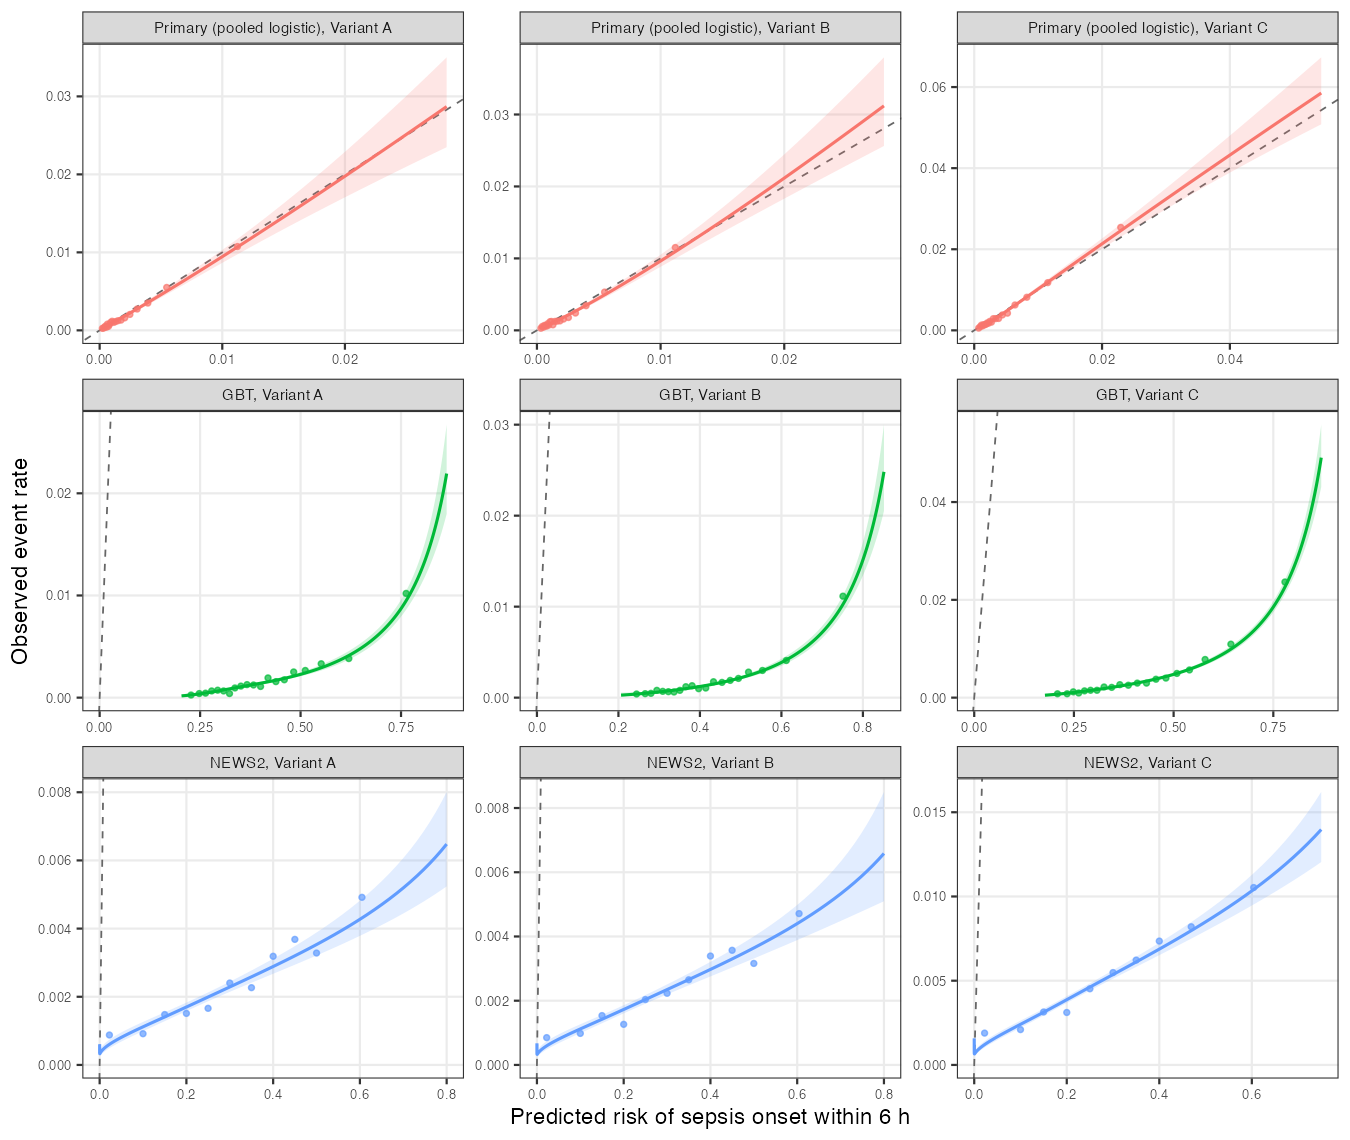
\includegraphics[width=\textwidth]{images/11_calibration_curves.png}
    \caption{Flexible calibration curves on the temporal test set. Dashed line
    = perfect calibration; points = twenty equal-sized bins of predicted risk;
    shaded band = 95\% confidence interval. Each panel has its own scale
    because the predicted-risk ranges differ by orders of magnitude.}
    \label{fig:calibration}
\end{figure}

\subsubsection{Sensitivity to the Probability Clamp}

Calibration is often computed after clamping predicted probabilities to
$[0.001, 0.999]$. That guard is standard for models whose predictions approach
0 or 1, but at a 0.2 per cent hourly event rate it distorts the estimate:
\pcPctBelowClampPrimaryA\% (Variant A),
\pcPctBelowClampPrimaryB\% (Variant B) and \pcPctBelowClampPrimaryC\%
(Variant C) of the primary model's predicted probabilities fall \emph{below}
the clamp floor, so the clamp overwrites a large share of the quantity being
measured. No predicted probability exceeds \pcMaxPredPrimaryC{} under any
variant, so only the floor binds. The values in Table~\ref{tab:calibration}
use a floor of $10^{-6}$. Under the conventional clamp the primary model's Variant A slope is
\pcCalibSlopeClampedPrimaryA{}, against \pcCalibSlopePrimaryA{} on the
$10^{-6}$ floor, so a calibration guard chosen without reference to the event
rate itself changes the reported estimate.

%===========================================================================


\section{Clinical Utility: Net Benefit, Operating Points, and Event-Level
    Detection}
\label{sec:clinical_utility}
%===========================================================================

This section reports four operational quantities: net benefit across a
plausible threshold range, the positive predictive value and false-alarm
rate at a fixed sensitivity, detection expressed per patient rather than per
person-hour, and the lead time gained when detection occurs.

Under the discrete-time competing-risks specification, $\text{event}=1$ marks
the onset hour itself, so each septic stay contributes one event hour out of a
mean of 45. Per-hour sensitivity requires the alert to fire \emph{in the onset
hour}; per-patient sensitivity asks only whether the patient was alerted before
onset. Per-hour figures alone understate detection and do not show the
associated alarm volume.

\subsection{Decision-Curve Analysis \texorpdfstring{[C]}{[C]}}

Decision-curve analysis requires a threshold grid, and at this prevalence the
choice of grid determines the result. A threshold probability of $t$ encodes a willingness to accept
$(1-t)/t$ false alarms per true detection. The hourly event rate here is
0.19--0.42 per cent, so the conventional grid of 0.01--0.20 sits between five
and one hundred times the prevalence: at $t=0.01$ the analyst is asserting a
tolerance of only 99 false alarms per detection, far below what an hourly
sepsis alert must absorb, and every curve falls trivially below ``treat
none''. Net benefit is therefore evaluated on a grid from one tenth to ten
times the prevalence, following Vickers and Elkin \cite{vickers2006dca}.

\begin{figure}[H]
    \centering
    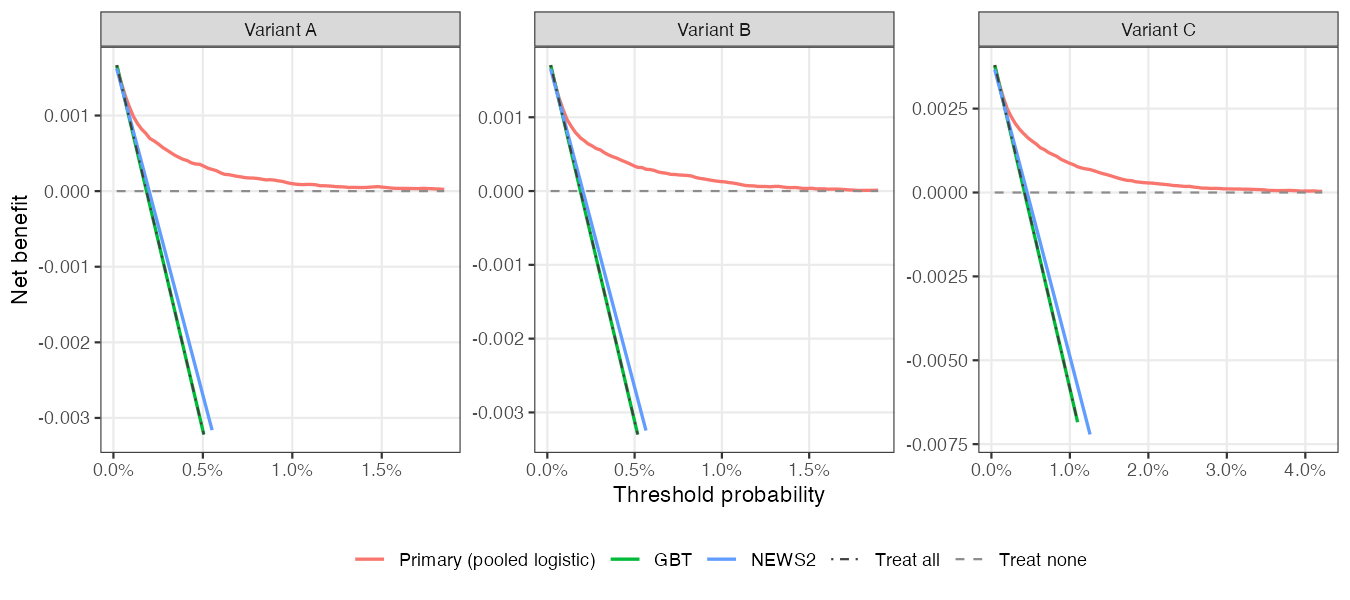
\includegraphics[width=\textwidth]{images/11_decision_curves.png}
    \caption{Decision curves on the temporal test set. Net benefit against
    threshold probability, with both default strategies shown. Curves are
    clipped below $-1.75\times$ prevalence for legibility.}
    \label{fig:decision_curves}
\end{figure}

\begin{table}[H]
    \centering\small
    \begin{tabular}{llrrrr}
        \toprule
        \textbf{Var} & \textbf{Model} & \textbf{Net benefit}
        & \textbf{Std NB} & \textbf{Alert rate} & \textbf{Alert-rate span} \\
        \midrule
        A & Primary & \pcNetBenefitPrimaryA & \pcSnbPrimaryA & \pcAlertRatePrimaryA & \pcAlertRangePrimaryA \\
        A & GBT     & \pcNetBenefitGbtA & \pcSnbGbtA & \pcAlertRateGbtA & \pcAlertRangeGbtA \\
        A & Cox     & \pcNetBenefitCoxA & \pcSnbCoxA & \pcAlertRateCoxA & \pcAlertRangeCoxA \\
        A & NEWS2   & \pcNetBenefitNewsA & \pcSnbNewsA & \pcAlertRateNewsA & \pcAlertRangeNewsA \\
        A & qSOFA   & \pcNetBenefitQsofaA & \pcSnbQsofaA & \pcAlertRateQsofaA & \pcAlertRangeQsofaA \\
        A & SIRS    & \pcNetBenefitSirsA & \pcSnbSirsA & \pcAlertRateSirsA & \pcAlertRangeSirsA \\
        \midrule
        B & Primary & \pcNetBenefitPrimaryB & \pcSnbPrimaryB & \pcAlertRatePrimaryB & \pcAlertRangePrimaryB \\
        B & GBT     & \pcNetBenefitGbtB & \pcSnbGbtB & \pcAlertRateGbtB & \pcAlertRangeGbtB \\
        B & Cox     & \pcNetBenefitCoxB & \pcSnbCoxB & \pcAlertRateCoxB & \pcAlertRangeCoxB \\
        B & NEWS2   & \pcNetBenefitNewsB & \pcSnbNewsB & \pcAlertRateNewsB & \pcAlertRangeNewsB \\
        B & qSOFA   & \pcNetBenefitQsofaB & \pcSnbQsofaB & \pcAlertRateQsofaB & \pcAlertRangeQsofaB \\
        B & SIRS    & \pcNetBenefitSirsB & \pcSnbSirsB & \pcAlertRateSirsB & \pcAlertRangeSirsB \\
        \midrule
        C & Primary & \pcNetBenefitPrimaryC & \pcSnbPrimaryC & \pcAlertRatePrimaryC & \pcAlertRangePrimaryC \\
        C & GBT     & \pcNetBenefitGbtC & \pcSnbGbtC & \pcAlertRateGbtC & \pcAlertRangeGbtC \\
        C & Cox     & \pcNetBenefitCoxC & \pcSnbCoxC & \pcAlertRateCoxC & \pcAlertRangeCoxC \\
        C & NEWS2   & \pcNetBenefitNewsC & \pcSnbNewsC & \pcAlertRateNewsC & \pcAlertRangeNewsC \\
        C & qSOFA   & \pcNetBenefitQsofaC & \pcSnbQsofaC & \pcAlertRateQsofaC & \pcAlertRangeQsofaC \\
        C & SIRS    & \pcNetBenefitSirsC & \pcSnbSirsC & \pcAlertRateSirsC & \pcAlertRangeSirsC \\
        \bottomrule
    \end{tabular}
    \caption{Net benefit at a threshold probability equal to the event
    prevalence. At that threshold both defaults have net benefit exactly zero
    and the maximum attainable net benefit is the prevalence itself, so
    standardised net benefit (Std NB = net benefit / prevalence) is the
    fraction of the attainable benefit captured. ``Alert-rate span'' is the
    change in alert rate across the threshold grid.}
    \label{tab:net_benefit}
\end{table}

Decision-curve analysis produced positive but modest net benefit for the
primary model. At a threshold equal to the prevalence, the primary model captures
\pcSnbPctPrimaryA\% (Variant A), \pcSnbPctPrimaryB\% (Variant B) and
\pcSnbPctPrimaryC\% (Variant C) of the attainable net benefit. The three
variants span barely three percentage points, so, unlike discrimination, this
share is insensitive to the reading of Sepsis-3. The qualitative result matches
the swept Utility Score (Table~\ref{tab:utility_optimum}): a small positive
margin for the fitted models and none for the rule-based comparators. The
magnitudes differ because the metrics price errors differently: net benefit
weights a false alarm by $t/(1-t)$, which at $t = \pcPrevalenceB$ is very
small, whereas the Utility Score imposes a fixed $-0.05$ penalty per
false-alert hour. Net benefit is therefore the more generous metric here, and
the gap widens as the alert rate rises. The preferred weighting of false alerts
depends on the intended clinical decision and should be specified before
deployment. This within-cohort disagreement is not an instance of H5's
internal-to-external estimand.

For every model except the primary one, the alert-rate span is zero across the
plausible threshold range. GBT and Cox alert on \emph{100\% of person-hours} at
every threshold in this range, so their decision curves coincide with treating
everyone (Figure~\ref{fig:decision_curves}); with predicted probabilities in
the 0.2--0.9 range (Table~\ref{tab:calibration}), no threshold below 4 per cent
excludes anything. NEWS2, qSOFA and SIRS are non-tunable for the opposite
reason: their integer scores map to a few fixed probabilities, all above the
grid, and they alert on a constant 58--86 per cent of person-hours. Within the
clinically plausible range, the primary model is therefore the only one whose
alert rate responds to the threshold; GBT's best operating point lies far above
that range (Table~\ref{tab:utility_optimum}).

\subsection{Operating Points at Fixed Sensitivity \texorpdfstring{[E]}{[E]}}
\label{sec:operating_points}

Alerting systems are usually commissioned by choosing a sensitivity target
rather than a fixed cut-off. Table~\ref{tab:operating_points} sets the threshold to the
largest cut-off achieving 80 per cent per-hour sensitivity and reads off the
resulting operating characteristics.

\begin{table}[H]
    \centering\small
    \adjustbox{max width=\textwidth}{%
    \begin{tabular}{llrrrrrr}
        \toprule
        \textbf{Var} & \textbf{Model} & \textbf{Specificity} & \textbf{PPV}
        & \textbf{NNE} & \textbf{Alerts/pt-day} & \textbf{FA/pt-day}
        & \textbf{FP:TP} \\
        \midrule
        A & Primary & \pcSpecPrimaryA & \pcPpvPrimaryA & \pcNnePrimaryA & \pcAlertsPerPtDayPrimaryA & \pcFaPerPtDayPrimaryA & \pcFpTpRatioPrimaryA \\
        A & GBT     & \pcSpecGbtA & \pcPpvGbtA & \pcNneGbtA & \pcAlertsPerPtDayGbtA & \pcFaPerPtDayGbtA & \pcFpTpRatioGbtA \\
        A & NEWS2   & \pcSpecNewsA & \pcPpvNewsA & \pcNneNewsA & \pcAlertsPerPtDayNewsA & \pcFaPerPtDayNewsA & \pcFpTpRatioNewsA \\
        A & Cox     & \pcSpecCoxA & \pcPpvCoxA & \pcNneCoxA & \pcAlertsPerPtDayCoxA & \pcFaPerPtDayCoxA & \pcFpTpRatioCoxA \\
        \midrule
        B & Primary & \pcSpecPrimaryB & \pcPpvPrimaryB & \pcNnePrimaryB & \pcAlertsPerPtDayPrimaryB & \pcFaPerPtDayPrimaryB & \pcFpTpRatioPrimaryB \\
        B & GBT     & \pcSpecGbtB & \pcPpvGbtB & \pcNneGbtB & \pcAlertsPerPtDayGbtB & \pcFaPerPtDayGbtB & \pcFpTpRatioGbtB \\
        B & NEWS2   & \pcSpecNewsB & \pcPpvNewsB & \pcNneNewsB & \pcAlertsPerPtDayNewsB & \pcFaPerPtDayNewsB & \pcFpTpRatioNewsB \\
        B & Cox     & \pcSpecCoxB & \pcPpvCoxB & \pcNneCoxB & \pcAlertsPerPtDayCoxB & \pcFaPerPtDayCoxB & \pcFpTpRatioCoxB \\
        \midrule
        C & Primary & \pcSpecPrimaryC & \pcPpvPrimaryC & \pcNnePrimaryC & \pcAlertsPerPtDayPrimaryC & \pcFaPerPtDayPrimaryC & \pcFpTpRatioPrimaryC \\
        C & GBT     & \pcSpecGbtC & \pcPpvGbtC & \pcNneGbtC & \pcAlertsPerPtDayGbtC & \pcFaPerPtDayGbtC & \pcFpTpRatioGbtC \\
        C & NEWS2   & \pcSpecNewsC & \pcPpvNewsC & \pcNneNewsC & \pcAlertsPerPtDayNewsC & \pcFaPerPtDayNewsC & \pcFpTpRatioNewsC \\
        C & Cox     & \pcSpecCoxC & \pcPpvCoxC & \pcNneCoxC & \pcAlertsPerPtDayCoxC & \pcFaPerPtDayCoxC & \pcFpTpRatioCoxC \\
        \bottomrule
    \end{tabular}}
    \caption{Operating characteristics at a fixed per-hour sensitivity of
    80\%. NNE = number needed to evaluate ($1/\text{PPV}$), the alerted
    person-hours required per true event hour. FA/pt-day = false-alert hours
    per patient-day. qSOFA and SIRS are reported separately in the text
    because they degenerate at this target.}
    \label{tab:operating_points}
\end{table}

At 80 per cent sensitivity, PPV never exceeds \pcPpvPrimaryC. The best case,
the primary model under the Liberal label, still requires \pcNnePrimaryC{}
alerted person-hours per true event hour; under the Seymour-Standard label the
same model requires \pcNnePrimaryB. Every configuration generates between
\pcFaPerPtDayPrimaryC{} and \pcFaPerPtDayNewsA{} false-alert hours per
patient-day; even the best configuration generates \pcFaPerPtDayPrimaryC{}
false-alert hours per patient-day.

This ordering differs from the AUROC ordering. The primary model and GBT are
separated by less than 0.02 AUROC (H6), but at a fixed sensitivity target the
primary model needs fewer alerts per true event under all three labels.

A sensitivity target also exposes the coarse rule-based scores. qSOFA
cannot be tuned to 80 per cent sensitivity under the Liberal label at all: with
only \pcNDistinctQsofa{} distinct score values, the lowest cut-off reaching the
target is the one that alerts on every person-hour (specificity \pcSpecQsofaC,
\pcFaPerPtDayQsofaC{} false-alert hours per patient-day). It reaches the target
under Variants A and B only at specificity \pcSpecQsofaA{} and
\pcFaPerPtDayQsofaA{} false-alert hours per patient-day.

\begin{figure}[H]
    \centering
    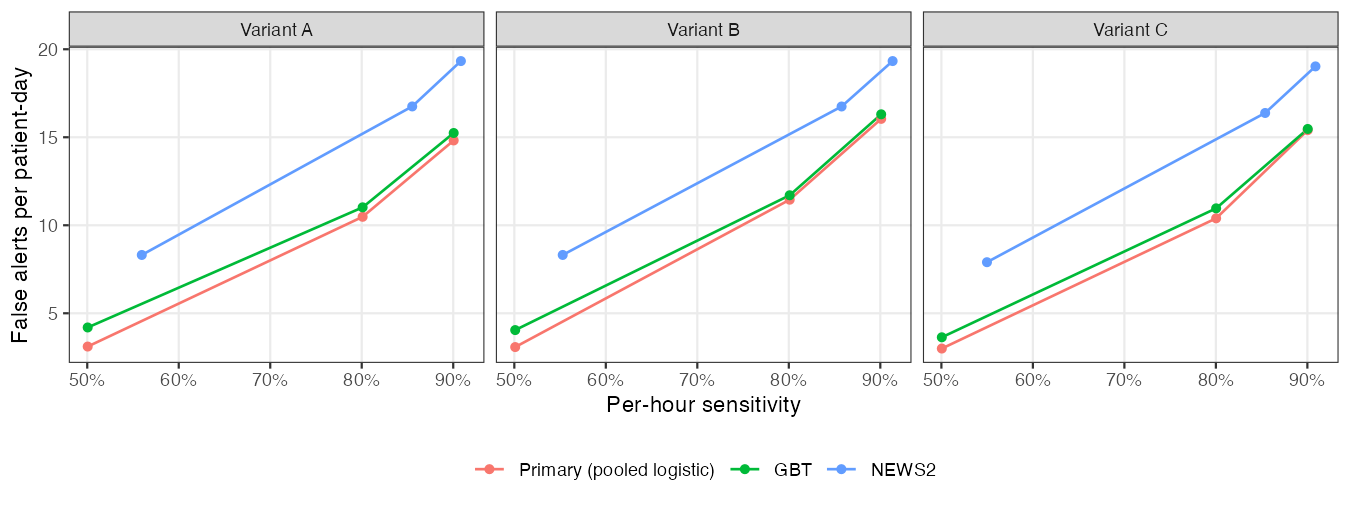
\includegraphics[width=\textwidth]{images/11_false_alarms_vs_sensitivity.png}
    \caption{False alerts per patient-day against per-hour sensitivity, at
    sensitivity targets of 50\%, 80\% and 90\%. The relationship is close to
    linear across the range.}
    \label{fig:fa_vs_sens}
\end{figure}

\subsection{Per-Patient (Event-Level) Detection \texorpdfstring{[C]}{[C]}}

Table~\ref{tab:patient_level} re-expresses the same operating points per
patient. Episode sensitivity within the actionable window counts a septic stay
as detected if any alert fired between six hours before onset and onset
itself. A false-alarm episode is a contiguous run of alert hours that does not
overlap the window from six hours before to three hours after onset, so a
five-hour alert run counts once rather than five times.

\begin{table}[H]
    \centering\small
    \adjustbox{max width=\textwidth}{%
    \begin{tabular}{llrrrrr}
        \toprule
        \textbf{Var} & \textbf{Model}
        & \textbf{Ep.\ sens (6\,h)} & \textbf{Ep.\ sens (any pre)}
        & \textbf{Patient PPV} & \textbf{\% stays alerted}
        & \textbf{FA ep./pt-day} \\
        \midrule
        A & Primary & \pcEpSensWindowPrimaryA & \pcEpSensPrePrimaryA & \pcPatientPpvPrimaryA & \pcPctStaysAlertedPrimaryA & \pcFaEpPerPtDayPrimaryA \\
        A & GBT     & \pcEpSensWindowGbtA & \pcEpSensPreGbtA & \pcPatientPpvGbtA & \pcPctStaysAlertedGbtA & \pcFaEpPerPtDayGbtA \\
        A & NEWS2   & \pcEpSensWindowNewsA & \pcEpSensPreNewsA & \pcPatientPpvNewsA & \pcPctStaysAlertedNewsA & \pcFaEpPerPtDayNewsA \\
        A & Cox     & \pcEpSensWindowCoxA & \pcEpSensPreCoxA & \pcPatientPpvCoxA & \pcPctStaysAlertedCoxA & \pcFaEpPerPtDayCoxA \\
        \midrule
        B & Primary & \pcEpSensWindowPrimaryB & \pcEpSensPrePrimaryB & \pcPatientPpvPrimaryB & \pcPctStaysAlertedPrimaryB & \pcFaEpPerPtDayPrimaryB \\
        B & GBT     & \pcEpSensWindowGbtB & \pcEpSensPreGbtB & \pcPatientPpvGbtB & \pcPctStaysAlertedGbtB & \pcFaEpPerPtDayGbtB \\
        B & NEWS2   & \pcEpSensWindowNewsB & \pcEpSensPreNewsB & \pcPatientPpvNewsB & \pcPctStaysAlertedNewsB & \pcFaEpPerPtDayNewsB \\
        B & Cox     & \pcEpSensWindowCoxB & \pcEpSensPreCoxB & \pcPatientPpvCoxB & \pcPctStaysAlertedCoxB & \pcFaEpPerPtDayCoxB \\
        \midrule
        C & Primary & \pcEpSensWindowPrimaryC & \pcEpSensPrePrimaryC & \pcPatientPpvPrimaryC & \pcPctStaysAlertedPrimaryC & \pcFaEpPerPtDayPrimaryC \\
        C & GBT     & \pcEpSensWindowGbtC & \pcEpSensPreGbtC & \pcPatientPpvGbtC & \pcPctStaysAlertedGbtC & \pcFaEpPerPtDayGbtC \\
        C & NEWS2   & \pcEpSensWindowNewsC & \pcEpSensPreNewsC & \pcPatientPpvNewsC & \pcPctStaysAlertedNewsC & \pcFaEpPerPtDayNewsC \\
        C & Cox     & \pcEpSensWindowCoxC & \pcEpSensPreCoxC & \pcPatientPpvCoxC & \pcPctStaysAlertedCoxC & \pcFaEpPerPtDayCoxC \\
        \bottomrule
    \end{tabular}}
    \caption{Per-patient detection at the 80\% per-hour sensitivity operating
    point, on \pcNTestStays{} test stays of which \pcNSepsisStaysA{} (A),
    \pcNSepsisStaysB{} (B) and \pcNSepsisStaysC{} (C) are septic. Ep.\ sens (6\,h): fraction of septic stays alerted
    within $[\text{onset}-6\,\text{h},\ \text{onset}]$. Ep.\ sens (any pre):
    alerted at any point before onset. FA ep./pt-day: false-alarm episodes,
    not alert-hours, per patient-day.}
    \label{tab:patient_level}
\end{table}

Under the primary label, \pcEpSensWindowPrimaryB{} of septic patients are
alerted inside the six-hour window and \pcEpSensPrePrimaryB{} at some point
before onset. Interpreted alone, patient-level detection obscures the
associated alert burden: to achieve it, the models alert on
\pcPctStaysAlertedCoxB--\pcPctStaysAlertedPrimaryA{} per cent of \emph{all}
stays. Patient-level PPV falls to \pcPatientPpvPrimaryB{} under Variant
B and \pcPatientPpvPrimaryC{} under Variant C, which are, to three decimal
places, the septic fractions of the cohort themselves
(\pcNSepsisStaysB/\pcNTestStays{} and
\pcNSepsisStaysC/\pcNTestStays). Because nearly every stay is alerted,
patient-level alerts provide little discrimination beyond the cohort
prevalence; under Variants A and C the primary model alerts on
\pcPctStaysAlertedPrimaryA{} per cent of the \pcNTestStays{} test stays.

\subsubsection{Per-Hour and Per-Patient, Side by Side}

\begin{table}[H]
    \centering\small
    \adjustbox{max width=\textwidth}{%
    \begin{tabular}{llrrrrrr}
        \toprule
        \textbf{Var} & \textbf{Model}
        & \textbf{Sens (hr)} & \textbf{Sens (pt)}
        & \textbf{PPV (hr)} & \textbf{PPV (pt)}
        & \textbf{FA hr/pt-day} & \textbf{FA ep./pt-day} \\
        \midrule
        A & Primary & \pcSensPrimaryA & \pcEpSensPrePrimaryA & \pcPpvPrimaryA & \pcPatientPpvPrimaryA & \pcFaPerPtDayPrimaryA & \pcFaEpPerPtDayPrimaryA \\
        A & GBT     & \pcSensGbtA & \pcEpSensPreGbtA & \pcPpvGbtA & \pcPatientPpvGbtA & \pcFaPerPtDayGbtA & \pcFaEpPerPtDayGbtA \\
        A & NEWS2   & \pcSensNewsA & \pcEpSensPreNewsA & \pcPpvNewsA & \pcPatientPpvNewsA & \pcFaPerPtDayNewsA & \pcFaEpPerPtDayNewsA \\
        \midrule
        B & Primary & \pcSensPrimaryB & \pcEpSensPrePrimaryB & \pcPpvPrimaryB & \pcPatientPpvPrimaryB & \pcFaPerPtDayPrimaryB & \pcFaEpPerPtDayPrimaryB \\
        B & GBT     & \pcSensGbtB & \pcEpSensPreGbtB & \pcPpvGbtB & \pcPatientPpvGbtB & \pcFaPerPtDayGbtB & \pcFaEpPerPtDayGbtB \\
        B & NEWS2   & \pcSensNewsB & \pcEpSensPreNewsB & \pcPpvNewsB & \pcPatientPpvNewsB & \pcFaPerPtDayNewsB & \pcFaEpPerPtDayNewsB \\
        \midrule
        C & Primary & \pcSensPrimaryC & \pcEpSensPrePrimaryC & \pcPpvPrimaryC & \pcPatientPpvPrimaryC & \pcFaPerPtDayPrimaryC & \pcFaEpPerPtDayPrimaryC \\
        C & GBT     & \pcSensGbtC & \pcEpSensPreGbtC & \pcPpvGbtC & \pcPatientPpvGbtC & \pcFaPerPtDayGbtC & \pcFaEpPerPtDayGbtC \\
        C & NEWS2   & \pcSensNewsC & \pcEpSensPreNewsC & \pcPpvNewsC & \pcPatientPpvNewsC & \pcFaPerPtDayNewsC & \pcFaEpPerPtDayNewsC \\
        \bottomrule
    \end{tabular}}
    \caption{The same operating point viewed per person-hour and per patient.
    Across these rows the two views differ by more than twentyfold in PPV and
    by roughly tenfold in alarm count.}
    \label{tab:hour_vs_patient}
\end{table}

Per-hour PPV of \pcPpvPrimaryB{} and per-patient PPV of
\pcPatientPpvPrimaryB{} describe one model at one threshold on one test set.
The choice of denominator changes the reported PPV by a factor of twenty-six,
more than the spread attributed to label definition (H1) or model class (H6),
so it is an analyst decision that requires pre-specification.

\subsection{Lead Time to Onset \texorpdfstring{[C]}{[C]}}

Lead time is the interval between the first alert issued at or before onset
and the onset hour, over septic stays that were alerted at all.

\begin{table}[H]
    \centering\small
    \begin{tabular}{llrrrr}
        \toprule
        \textbf{Var} & \textbf{Model} & \textbf{Median (h)} & \textbf{IQR (h)}
        & \textbf{$\geq 3$\,h} & \textbf{$\geq 6$\,h} \\
        \midrule
        A & Primary & \pcLeadMedianPrimaryA & \pcLeadQXXVPrimaryA--\pcLeadQLXXVPrimaryA & \pcFracLeadGeThreePrimaryA & \pcFracLeadGeSixPrimaryA \\
        A & GBT     & \pcLeadMedianGbtA & \pcLeadQXXVGbtA--\pcLeadQLXXVGbtA & \pcFracLeadGeThreeGbtA & \pcFracLeadGeSixGbtA \\
        A & NEWS2   & \pcLeadMedianNewsA & \pcLeadQXXVNewsA--\pcLeadQLXXVNewsA & \pcFracLeadGeThreeNewsA & \pcFracLeadGeSixNewsA \\
        A & Cox     & \pcLeadMedianCoxA & \pcLeadQXXVCoxA--\pcLeadQLXXVCoxA & \pcFracLeadGeThreeCoxA & \pcFracLeadGeSixCoxA \\
        \midrule
        B & Primary & \pcLeadMedianPrimaryB & \pcLeadQXXVPrimaryB--\pcLeadQLXXVPrimaryB & \pcFracLeadGeThreePrimaryB & \pcFracLeadGeSixPrimaryB \\
        B & GBT     & \pcLeadMedianGbtB & \pcLeadQXXVGbtB--\pcLeadQLXXVGbtB & \pcFracLeadGeThreeGbtB & \pcFracLeadGeSixGbtB \\
        B & NEWS2   & \pcLeadMedianNewsB & \pcLeadQXXVNewsB--\pcLeadQLXXVNewsB & \pcFracLeadGeThreeNewsB & \pcFracLeadGeSixNewsB \\
        B & Cox     & \pcLeadMedianCoxB & \pcLeadQXXVCoxB--\pcLeadQLXXVCoxB & \pcFracLeadGeThreeCoxB & \pcFracLeadGeSixCoxB \\
        \midrule
        C & Primary & \pcLeadMedianPrimaryC & \pcLeadQXXVPrimaryC--\pcLeadQLXXVPrimaryC & \pcFracLeadGeThreePrimaryC & \pcFracLeadGeSixPrimaryC \\
        C & GBT     & \pcLeadMedianGbtC & \pcLeadQXXVGbtC--\pcLeadQLXXVGbtC & \pcFracLeadGeThreeGbtC & \pcFracLeadGeSixGbtC \\
        C & NEWS2   & \pcLeadMedianNewsC & \pcLeadQXXVNewsC--\pcLeadQLXXVNewsC & \pcFracLeadGeThreeNewsC & \pcFracLeadGeSixNewsC \\
        C & Cox     & \pcLeadMedianCoxC & \pcLeadQXXVCoxC--\pcLeadQLXXVCoxC & \pcFracLeadGeThreeCoxC & \pcFracLeadGeSixCoxC \\
        \bottomrule
    \end{tabular}
    \caption{Lead time at the 80\% sensitivity operating point. The
    $\geq 3$\,h and $\geq 6$\,h columns are fractions of \emph{all} septic
    stays, not only detected ones.}
    \label{tab:lead_time}
\end{table}

\begin{figure}[H]
    \centering
    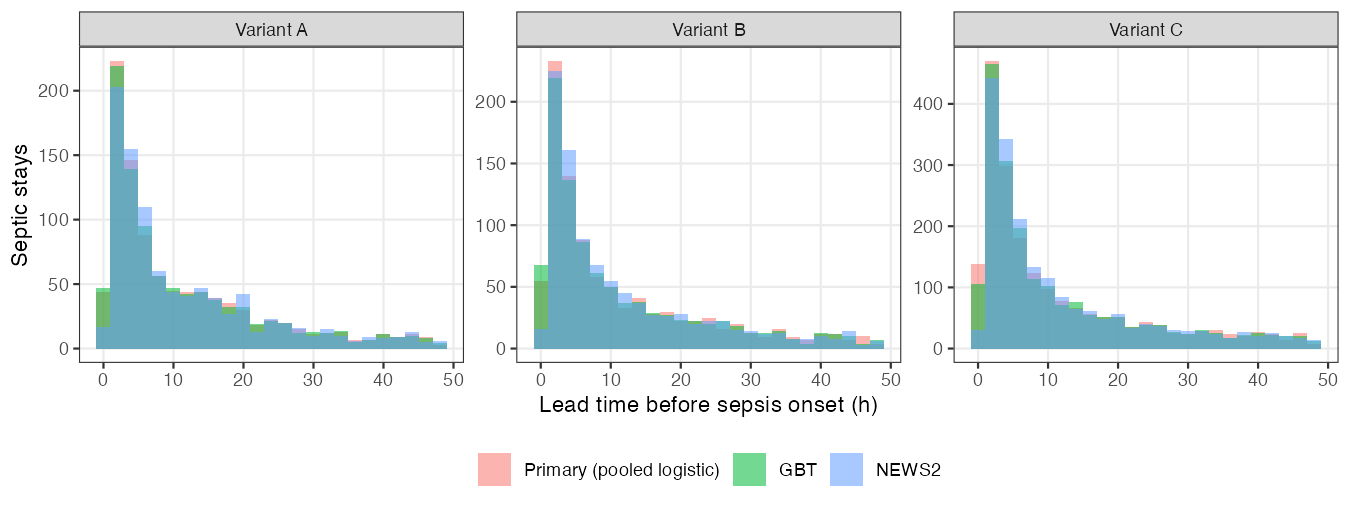
\includegraphics[width=\textwidth]{images/11_lead_time_distribution.png}
    \caption{Distribution of lead time before onset at the 80\% sensitivity
    operating point, truncated at 48 h. The mode lies in the first four hours,
    with a long right tail. Because almost every stay is alerted at this
    operating point, the distribution is not evidence of advance warning.}
    \label{fig:lead_time}
\end{figure}

Median lead time is \pcLeadMedianPrimaryC--\pcLeadMedianPrimaryB{} hours for
the primary model, with \pcFracLeadGeSixPrimaryB{} of septic stays alerted at
least six hours ahead under the primary label, but nearly every stay is
alerted at this operating point. The long lead-time tail
(Figure~\ref{fig:lead_time}) therefore includes alerts unrelated to the
subsequent onset, and these estimates are not comparable with the 4--12 hour
horizons in the literature \cite{henry2015trewscore, moor2023review}. They
should not be interpreted as evidence of actionable advance warning without
controlling alert burden.

%===========================================================================


\section{External Validation on eICU-CRD \texorpdfstring{[C]}{[C]}}
\label{sec:external_validation}
\label{sec:external}
%===========================================================================

External validation asks whether a frozen model ranks person-hours as well in a
different health system as in the one it was fitted on. Because the Sepsis-3
label must be transported as well as the model, this section reports the
labelling inputs first, then discrimination, then operating characteristics.

\subsection{Coverage of the Sepsis-3 Anchor in eICU-CRD}
\label{sec:external_coverage}

In eICU-CRD the culture limb of the Sepsis-3 anchor is documented for
\pcExtMicroCoverage\% of the analysis cohort (\pcExtNMicroStays{} of
\pcExtNCohortStays{} unit stays), whereas antibiotic exposure, pooled across
the \texttt{medication} and \texttt{infusionDrug} tables, reaches
\pcExtAbxCoverage\% of stays. Both limbs are documented at any offset for
\pcExtNBothLimbStays{} stays (\pcExtBothLimbCoverage\%); they co-occur inside
each variant's antibiotic--culture window for \pcExtNSuspicionA{},
\pcExtNSuspicionB{} and \pcExtNSuspicionC{} stays under Variants A, B and C;
and adding the organ-dysfunction criterion leaves \pcExtNOnsetStaysA{},
\pcExtNOnsetStaysB{} and \pcExtNOnsetStaysC{} labelled stays.

Under Variant B, \pcExtNOnsetStaysB{} stays are labelled but \pcExtNEventsB{}
events are scored: an onset after a stay's last observed hour is treated as
right-censoring, the horizon rule the development cohort applies at 72 hours.
Two of Variant B's onsets fall this way and none of Variant A's or C's; every
other labelled onset hour receives a prediction from all three models.

Because no onset is observable in a stay without a culture record, the primary
external analysis is restricted to the \pcExtPanelHoursMicro{} person-hours of
the microbiology-covered sub-cohort rather than all \pcExtPanelHoursFull{}.
Table~\ref{tab:external_rates} reconciles the resulting event rates with the
development cohort's.

\begin{table}[H]
    \centering\small
    \adjustbox{max width=\textwidth}{%
    \begin{tabular}{llrrr}
        \toprule
        \textbf{Var} & \textbf{Cohort} & \textbf{Person-hours}
        & \textbf{Events} & \textbf{Events / 1{,}000 person-h} \\
        \midrule
        A & MIMIC-IV temporal test        & \pcNTestRowsA & \pcNTestEventsA & \pcExtRateMimicA \\
        A & eICU, microbiology-covered    & \pcExtNRowsA  & \pcExtNEventsA  & \pcExtRateEicuA \\
        A & eICU, antibiotic-only anchor  & \pcExtAbxNRowsA & \pcExtAbxNEventsA & \pcExtRateEicuAbxA \\
        \midrule
        B & MIMIC-IV temporal test        & \pcNTestRowsB & \pcNTestEventsB & \pcExtRateMimicB \\
        B & eICU, microbiology-covered    & \pcExtNRowsB  & \pcExtNEventsB  & \pcExtRateEicuB \\
        B & eICU, antibiotic-only anchor  & \pcExtAbxNRowsB & \pcExtAbxNEventsB & \pcExtRateEicuAbxB \\
        \midrule
        C & MIMIC-IV temporal test        & \pcNTestRowsC & \pcNTestEventsC & \pcExtRateMimicC \\
        C & eICU, microbiology-covered    & \pcExtNRowsC  & \pcExtNEventsC  & \pcExtRateEicuC \\
        C & eICU, antibiotic-only anchor  & \pcExtAbxNRowsC & \pcExtAbxNEventsC & \pcExtRateEicuAbxC \\
        \bottomrule
    \end{tabular}}
    \caption{Event-rate reconciliation for the development cohort and both
    external anchors. The antibiotic-only anchor is not Sepsis-3 and its rate
    is not interchangeable with the other two.}
    \label{tab:external_rates}
\end{table}

On the restricted cohort the external event rate is \pcExtRateEicuB{} per
thousand person-hours against MIMIC-IV's \pcExtRateMimicB{} under the primary
label, a ratio of \pcExtRateRatioB. Relaxing the culture requirement raises it
to \pcExtRateEicuAbxB{} per thousand (ratio \pcExtRateRatioAbxB), suggesting
that much of the gap lies in the culture limb. The residual includes case mix,
charting frequency and differences in illness severity;
Section~\ref{sec:external_altlabel} narrows it further by removing the anchor
altogether. A gap of two or more orders of magnitude between two large adult
ICU populations would be far more consistent with missing labelling inputs
than with a difference in incidence, and would call for an audit of those
inputs before the rate is interpreted.

\subsection{Discrimination Under Transport}

\begin{table}[H]
    \centering
    \adjustbox{max width=\textwidth}{%
    \begin{tabular}{llrrrr}
        \toprule
        \textbf{Var} & \textbf{Model} & \textbf{N rows} & \textbf{N events}
        & \textbf{AUROC (eICU)} & \textbf{AUROC (MIMIC)} \\
        \midrule
        A & Primary & \pcExtNRowsA & \pcExtNEventsA & \pcExtAurocPrimaryA & \pcAurocPrimaryA \\
        A & GBT     & \pcExtNRowsA & \pcExtNEventsA & \pcExtAurocGbtA  & \pcAurocGbtA \\
        A & NEWS2   & \pcExtNRowsA & \pcExtNEventsA & \pcExtAurocNewsA & \pcAurocNewsA \\
        \midrule
        B & Primary & \pcExtNRowsB & \pcExtNEventsB & \pcExtAurocPrimaryB & \pcAurocPrimaryB \\
        B & GBT     & \pcExtNRowsB & \pcExtNEventsB & \pcExtAurocGbtB  & \pcAurocGbtB \\
        B & NEWS2   & \pcExtNRowsB & \pcExtNEventsB & \pcExtAurocNewsB & \pcAurocNewsB \\
        \midrule
        C & Primary & \pcExtNRowsC & \pcExtNEventsC & \pcExtAurocPrimaryC & \pcAurocPrimaryC \\
        C & GBT     & \pcExtNRowsC & \pcExtNEventsC & \pcExtAurocGbtC  & \pcAurocGbtC \\
        C & NEWS2   & \pcExtNRowsC & \pcExtNEventsC & \pcExtAurocNewsC & \pcAurocNewsC \\
        \bottomrule
    \end{tabular}}
    \caption{External validation on eICU-CRD (frozen models, no retraining),
    Sepsis-3 anchor on the microbiology-covered sub-cohort. Each variant
    carries its own external label set, so the row counts and event counts
    differ across variants as they do internally.}
    \label{tab:external}
\end{table}

\textbf{The point estimate falls under every label.} The primary
model falls from \pcAurocPrimaryA{} to \pcExtAurocPrimaryA{} (Narrow), from
\pcAurocPrimaryB{} to \pcExtAurocPrimaryB{} (Seymour-Standard) and from
\pcAurocPrimaryC{} to \pcExtAurocPrimaryC{} (Liberal). Only the
Seymour-Standard contrast, the tested contrast of H5, carries an interval, and
it covers zero (Section~\ref{sec:h5}); the Narrow and Liberal figures are point
estimates on \pcExtNEventsA{} and \pcExtNEventsC{} events, so the three
indicate a direction rather than three established degradations. The
Seymour-Standard drop of \pcHFiveEst{} is about three-quarters of the 0.085
reference estimate reported by Moor et al.\ \cite{moor2023review}. The point
estimates show the same cross-label ordering as the internal results, although
the low event counts preclude interpreting that ordering.

NEWS2 falls to \pcExtAurocNewsB{} under the primary label, close to chance. On
this arm the fitted models therefore retain more of their advantage over a
bedside score, although under the antibiotic-only anchor, with two orders of
magnitude more events, the ordering between the boosted model and NEWS2 does
not hold (Section~\ref{sec:external_interpretability}).

The differing event counts and NEWS2 AUROCs across variants are consistent
with variant-specific external labels: NEWS2's score is label-invariant, but
its AUROC depends on the outcome it is ranked against.

Every external event count above falls below the interpretability floor
(Section~\ref{sec:external_interpretability}).

\subsection{The Anchor-Independent Label on the Full External Cohort
\texorpdfstring{[D]}{[D]}}
\label{sec:external_altlabel}

The estimates above are computed on the \pcExtNMicroStays{} stays
(\pcExtMicroCoverage\%) with documented microbiology. Variant D carries no
treatment timestamp, so it can be constructed on the whole cohort. This
subsection reports the frozen Variant D models applied to all
\pcExtAltNStays{} eICU-CRD stays under Protocol Amendment~9.

\begin{table}[H]
    \centering\small
    \begin{tabular}{lrrlr}
        \toprule
        \textbf{Model} & \textbf{Internal AUROC} & \textbf{External AUROC}
        & \textbf{Drop (95\% CI)} & \textbf{Events} \\
        \midrule
        Primary & \pcAltAurocFullPrimaryD & \pcExtAltAurocPrimary & \pcExtAltDropPrimary{} \pcExtAltDropCiPrimary & \pcExtAltNEvents \\
        GBT     & \pcAltAurocFullGbtD     & \pcExtAltAurocGbt     & \pcExtAltDropGbt{} \pcExtAltDropCiGbt & \pcExtAltNEvents \\
        NEWS2   & \pcNotApplicable        & \pcExtAltAurocNews    & \pcNotApplicable & \pcExtAltNEvents \\
        \bottomrule
    \end{tabular}
    \caption[Variant D on the full eICU-CRD cohort]{Variant D applied to all
    \pcExtAltNStays{} eICU-CRD stays (\pcExtAltNRows{} person-hours). The target
    is acute organ dysfunction, not Sepsis-3, so these values are not pooled
    with the Sepsis-3 arm. eICU-CRD's periodic vitals carry no Glasgow Coma
    Scale, so the external SOFA delta rests on five components against
    MIMIC-IV's six. The drop's interval resamples the two databases
    independently and differences the streams, as for H5 (Protocol
    Amendment~10). Post-hoc under Protocol Amendment~9; excluded from H5.}
    \label{tab:external_altlabel}
\end{table}

The arm scores \pcExtAltNEvents{} events over \pcExtAltNRows{} person-hours,
against \pcExtNEventsB{} under Variant B, and is the only external estimate that
clears the \pcExtMinEvents-event interpretability floor
(Section~\ref{sec:external_interpretability}).

\textbf{AUROC drop.} The primary
model falls from \pcAltAurocFullPrimaryD{} internally to
\pcExtAltAurocPrimary{} externally, a difference of
\pcExtAltDropPrimary{} (95\% CI \pcExtAltDropCiPrimary), and the
gradient-boosted comparator from
\pcAltAurocFullGbtD{} to \pcExtAltAurocGbt, a difference of
\pcExtAltDropGbt{} (\pcExtAltDropCiGbt). Both drops are of the order of the
0.085 degradation Moor et al.\ \cite{moor2023review} report across four
databases, and of the same order as the H5 estimate. The event count affects
the width rather than the location: both intervals exclude zero and are
narrower than a hundredth of a point, whereas H5's substituted contrast,
\pcHFiveEst{} [\pcHFiveCiLo, \pcHFiveCiHi] on \pcExtNEventsB{} events, is
compatible with both no degradation and a degradation twice as large. For the
deterioration target, transport between these databases therefore reduces
discrimination; this is not evidence about the Sepsis-3 target, a different
estimand.

\textbf{Event rate.} Under the Sepsis-3 anchor the external event rate is
\pcExtRateRatioB{} of the development cohort's, a gap of roughly an order of
magnitude located largely in the culture limb
(Section~\ref{sec:external_coverage}). Under the anchor-independent label the
two databases give \pcExtAltRateMimic{} and \pcExtAltRateEicu{} events per
1{,}000 person-hours, a ratio of \pcExtAltRateRatio. The reduction in the
event-rate gap after removing the treatment anchor suggests that label
transport accounts for a substantial part of the original discrepancy
(Section~\ref{sec:variant_d_establishes}).

\subsection{External Clinical Utility on eICU-CRD \texorpdfstring{[C]}{[C]}}

Operating characteristics are reported on the same microbiology-covered
sub-cohort and inherit its coverage limitation
(Section~\ref{sec:external_coverage}).

\begin{table}[H]
    \centering\small
    \begin{tabular}{llrrrrr}
        \toprule
        \textbf{Var} & \textbf{Model} & \textbf{Specificity} & \textbf{PPV}
        & \textbf{NNE} & \textbf{FA/pt-day} & \textbf{Patient PPV} \\
        \midrule
        A & Primary & \pcExtSpecPrimaryA & \pcExtPpvPrimaryA & \pcExtNnePrimaryA & \pcExtFaPerPtDayPrimaryA & \pcExtPatientPpvPrimaryA \\
        B & Primary & \pcExtSpecPrimaryB & \pcExtPpvPrimaryB & \pcExtNnePrimaryB & \pcExtFaPerPtDayPrimaryB & \pcExtPatientPpvPrimaryB \\
        C & Primary & \pcExtSpecPrimaryC & \pcExtPpvPrimaryC & \pcExtNnePrimaryC & \pcExtFaPerPtDayPrimaryC & \pcExtPatientPpvPrimaryC \\
        \midrule
        A--C & NEWS2 & \pcExtSpecNewsB & \pcExtPpvNewsB & \pcExtNneNewsB & \pcExtFaPerPtDayNewsB & \pcExtPatientPpvNewsB \\
        \bottomrule
    \end{tabular}
    \caption{eICU-CRD operating characteristics at the same 80\% target
    sensitivity, thresholds re-derived on the external cohort. All rows are
    drawn from the same \pcExtNStays{} microbiology-covered stays, but each
    variant carries its own label and therefore its own denominator:
    \pcExtNRowsA, \pcExtNRowsB{} and \pcExtNRowsC{} person-hours on
    \pcExtNEventsA, \pcExtNEventsB{} and \pcExtNEventsC{} event hours under
    A, B and C (Table~\ref{tab:external}). The NEWS2 row is scored under
    Variant B. Re-deriving thresholds externally excludes the further loss a
    threshold transported from MIMIC-IV would incur.}
    \label{tab:external_utility}
\end{table}

Operating characteristics on eICU-CRD are substantially worse than internal ones
at the same target sensitivity. Reaching 80 per cent sensitivity requires
\pcExtNnePrimaryC{} to \pcExtNnePrimaryA{} alerted person-hours per true event
hour, at \pcExtFaPerPtDayPrimaryB--\pcExtFaPerPtDayPrimaryA{} false-alert hours
per patient-day, roughly one alert every two hours per patient. NEWS2 cannot
reach the target without alerting on nearly
every person-hour (specificity \pcExtSpecNewsB, \pcExtFaPerPtDayNewsB{}
false-alert hours per patient-day). Patient-level PPV of
\pcExtPatientPpvPrimaryB{} is again the cohort septic fraction
(\pcExtNSepsisStays/\pcExtNStays), because the model alerts on essentially
every stay. At this event count the contributions of model and label cannot be
separated, since PPV, NNE and false-alarm rate all scale with the event rate;
these figures are therefore reported as an upper bound on transferability and
support no separate conclusion.

%===========================================================================


\section{Label-Anchor Attribution \texorpdfstring{[E]}{[E]}}
\label{sec:label_anchor_results}
%===========================================================================

Variants A, B and C vary the label within Sepsis-3 and share the
culture-plus-antibiotic anchor, so H1 cannot distinguish an effect of reading
the definition differently (definitional) from an effect of choosing a
different construct (empirical). This section separates the two by labelling
each limb of the Sepsis-3 conjunction separately (Section~\ref{sec:alt_labels};
post-hoc, Protocol Amendment 2, exploratory family E3).

\subsection{The Anchor Determines Every Onset Time}

Under Variants A, B and C the onset time is the suspicion time
$t_{\text{susp}}$; the SOFA criterion determines only \emph{whether} a stay is
labelled, not \emph{when}. Variant E, which removes the SOFA criterion, is
therefore a strict superset of Variant B: every one of B's
\pcNPositiveBPanel{} labelled stays is also labelled by E, and in
\textbf{\pcPctExactMatchE\% of them the onset hour is identical}. Adding the
organ-dysfunction requirement discards \pcNPositiveEExcessOverB{} of E's
\pcNPositiveE{} labelled stays, two thirds, and moves not one onset
by a single hour.

\begin{table}[H]
    \centering\small
    \adjustbox{max width=\textwidth}{%
    \begin{tabular}{llrrrrr}
        \toprule
        \textbf{Var} & \textbf{Label} & \textbf{Onsets ($\leq$72\,h)} & \textbf{\%}
        & \textbf{$\kappa$ vs B} & \textbf{Sens.\ to B}
        & \textbf{Exact onset match} \\
        \midrule
        A & Narrow          & \pcNPositiveA  & \pcPctOnsetsAPanel  & \pcKappaVsBA & \pcSensToBA & \pcPctExactMatchA\% \\
        B & Seymour-Std     & \pcNPositiveBPanel & \pcPctOnsetsBPanel & n/a   & n/a   & n/a    \\
        C & Liberal         & \pcNPositiveC  & \pcPctOnsetsCPanel  & \pcKappaVsBC & \pcSensToBC & \pcPctExactMatchC\% \\
        \midrule
        E & Anchor-Only     & \pcNPositiveE  & \pcPctOnsetsEPanel  & \pcKappaVsBE & \textbf{\pcSensToBE} & \textbf{\pcPctExactMatchE\%} \\
        D & Deterioration   & \pcNPositiveD  & \pcPctOnsetsDPanel  & \textbf{\pcKappaVsBD} & \pcSensToBD & \textbf{\pcPctExactMatchD\%} \\
        F & Sepsis-3 Early  & \pcNPositiveF  & \pcPctOnsetsFPanel  & \pcKappaVsBF & \textbf{\pcSensToBF} & \pcPctExactMatchF\% \\
        \bottomrule
    \end{tabular}}
    \caption{Onset agreement with Variant B across all five comparison variants,
    on the \pcNStays{} shared stays. Counts are restricted to onsets inside the
    72\,h modelling horizon so that Variant D, whose onsets exist only within the
    panel, is comparable. ``Sens.\ to B'' is the fraction of B's labelled stays
    that the variant also labels; ``exact onset match'' is computed among stays
    labelled by both.}
    \label{tab:label_agreement}
\end{table}

Within Sepsis-3 (Table~\ref{tab:label_agreement}, top block), variants that
agree a stay is septic almost always agree on the hour: \pcPctExactMatchA\% for A, \pcPctExactMatchC\%
for C. The pre-registered label variance therefore concerns \emph{which
patients} rather than \emph{when}, since timing is fixed by the treatment anchor
in all three. That disagreement is substantial: A and B share only \pcSensToBA{} of B's septic stays
($\kappa = \pcKappaVsBA$) despite near-identical prevalence.

A label built from physiology alone (Variant D) agrees with Sepsis-3 at $\kappa = \pcKappaVsBD$, barely distinguishable from
chance, and matches B's exact onset hour in only \pcPctExactMatchD\% of the
stays both label, with a median absolute shift of \pcMedianAbsShiftHD\,hours
(IQR \pcIqrShiftLoHD{} to $+\pcIqrShiftHiHD$). The anchor-independent label
thus identifies largely different patients at different times.

Variant F keeps the construct and the patients but changes the onset timing.
It labels every stay B labels ($\kappa = \pcKappaVsBF$, the
shortfall being the \pcFNExtraInHorizon{} stays discussed above whose onset only
enters the horizon under the earlier rule) yet agrees with B on the exact hour
in just \pcPctExactMatchF\% of them: two defensible readings of the same
definition place about a quarter of Sepsis-3 onsets at a different hour on the
same patients.

\subsection{Discrimination Under Each Limb}

\begin{table}[H]
    \centering\small
    \begin{tabular}{lrrrr@{\hskip 1.5em}rrrr}
        \toprule
        & \multicolumn{4}{c}{\textbf{AUROC}} & \multicolumn{4}{c}{\textbf{AUPRC}} \\
        \cmidrule(lr){2-5}\cmidrule(lr){6-9}
        \textbf{Model} & \textbf{B} & \textbf{E} & \textbf{D} & \textbf{F}
                       & \textbf{B} & \textbf{E} & \textbf{D} & \textbf{F} \\
        \midrule
        Primary & \pcAurocPrimaryB & \pcAltAurocFullPrimaryE & \pcAltAurocFullPrimaryD & \pcAltAurocFullPrimaryF
                & \pcAuprcPrimaryB & \pcAltAuprcFullPrimaryE & \pcAltAuprcFullPrimaryD & \pcAltAuprcFullPrimaryF \\
        GBT     & \pcAurocGbtB     & \pcAltAurocFullGbtE     & \pcAltAurocFullGbtD     & \pcAltAurocFullGbtF
                & \pcAuprcGbtB     & \pcAltAuprcFullGbtE     & \pcAltAuprcFullGbtD     & \pcAltAuprcFullGbtF \\
        NEWS2   & \pcAurocNewsB    & \pcAltAurocFullNewsE    & \pcAltAurocFullNewsD    & \pcAltAurocFullNewsF
                & \pcAuprcNewsB    & \pcAltAuprcFullNewsE    & \pcAltAuprcFullNewsD    & \pcAltAuprcFullNewsF \\
        Cox     & \pcAurocCoxB     & \pcAltAurocFullCoxE     & \pcAltAurocFullCoxD     & \pcAltAurocFullCoxF
                & \pcAuprcCoxB     & \pcAltAuprcFullCoxE     & \pcAltAuprcFullCoxD     & \pcAltAuprcFullCoxF \\
        qSOFA   & \pcAurocQsofaB   & \pcAltAurocFullQsofaE   & \pcAltAurocFullQsofaD   & \pcAltAurocFullQsofaF
                & \pcAuprcQsofaB   & \pcAltAuprcFullQsofaE   & \pcAltAuprcFullQsofaD   & \pcAltAuprcFullQsofaF \\
        SIRS    & \pcAurocSirsB    & \pcAltAurocFullSirsE    & \pcAltAurocFullSirsD    & \pcAltAurocFullSirsF
                & \pcAuprcSirsB    & \pcAltAuprcFullSirsE    & \pcAltAuprcFullSirsD    & \pcAltAuprcFullSirsF \\
        \midrule
        \textbf{Events} & \pcNTestEventsB & \pcAltNEventsE & \pcAltNEventsD & \pcAltNEventsF & & & & \\
        \bottomrule
    \end{tabular}
    \caption{Discrimination under each limb of the Sepsis-3 conjunction and
    under standard onset timing (temporal test set, unrestricted window).
    B = Sepsis-3 (anchor \textbf{and} organ dysfunction); E = suspicion anchor
    only; D = organ dysfunction only, anchor-independent; F = Sepsis-3 with
    onset at $\min(t_{\text{susp}}, t_{\text{SOFA}})$. AUPRC is reported
    alongside AUROC because the four labels have very different prevalences.}
    \label{tab:label_anchor}
\end{table}

\begin{figure}[H]
    \centering
    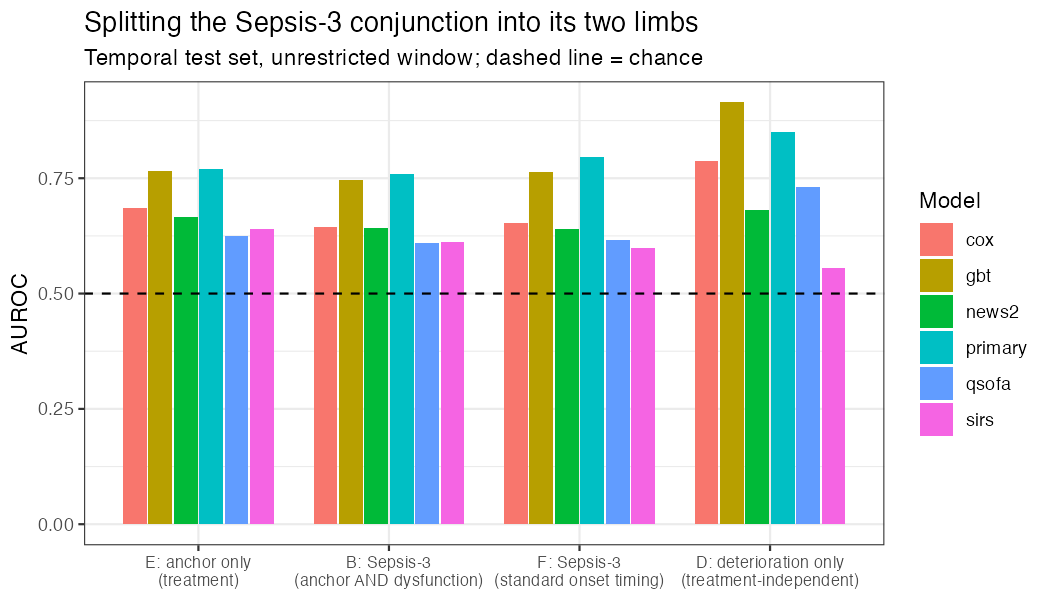
\includegraphics[width=0.9\textwidth]{images/09_label_anchor_attribution.png}
    \caption{Splitting the Sepsis-3 conjunction. The two limbs and the intact
    conjunction sit close together; only the anchor-independent deterioration
    label separates from them, and its level is not comparable with the others
    (Section~\ref{sec:variant_d_establishes}). The dashed line is chance.}
    \label{fig:label_anchor}
\end{figure}

\paragraph{Anchor-attributable fraction.}
The share of Sepsis-3's above-chance discrimination that the treatment anchor
reproduces on its own (Equation~\ref{eq:anchor_fraction}), with the ratio
bootstrapped end to end, is
\[
    \phi_{\text{anchor}} = \pcPhiAnchorPrimary
    \;\;[\pcPhiAnchorCiLoPrimary,\, \pcPhiAnchorCiHiPrimary]
    \quad\text{(primary)},\qquad
    \pcPhiAnchorGbt
    \;\;[\pcPhiAnchorCiLoGbt,\, \pcPhiAnchorCiHiGbt]
    \quad\text{(GBT)}.
\]
For the primary model the interval \textbf{includes 1}, and the underlying
contrast is not significant: E against B is
$\Delta = \pcAltDeltaPrimaryE$ [\pcAltDeltaCiLoPrimaryE,
\pcAltDeltaCiHiPrimaryE], $p_{\text{BH}} = \pcAltDeltaPBhPrimaryE$ in family E3.
For GBT the interval sits just above 1 ($\Delta = \pcAltDeltaGbtE$,
$p_{\text{BH}} = \pcAltDeltaPBhGbtE$), a small but detectable effect.

On this cohort the treatment anchor alone is therefore about as predictable as
Sepsis-3 itself. Dropping the organ-dysfunction requirement nearly triples the
event count (\pcAltNEventsE{} against \pcNTestEventsB) and leaves
discrimination essentially unchanged: the SOFA gate selects which stays are
labelled without selecting the more separable ones.

\paragraph{Anchor-independent label.}
Variant D differs substantially: $\Delta = \pcAltDeltaPrimaryD$
[\pcAltDeltaCiLoPrimaryD, \pcAltDeltaCiHiPrimaryD] for the primary model and
$\pcAltDeltaGbtD$ for GBT, both significant in family E3. Its AUPRC gap is
larger still (\pcAltAuprcFullPrimaryD{} against \pcAuprcPrimaryB), which matters
more at this prevalence. Because five of D's six SOFA components are model
inputs, part of this separation is self-fulfilling
(Section~\ref{sec:alt_labels}).

\paragraph{Onset timing.}
Variant F, whose label is Sepsis-3 unmodified in membership, is also
significantly more separable than B ($\Delta = \pcAltDeltaPrimaryF$
[\pcAltDeltaCiLoPrimaryF, \pcAltDeltaCiHiPrimaryF],
$p_{\text{BH}} = \pcAltDeltaPBhPrimaryF$). Its AUPRC is \emph{higher} than B's
despite a comparable event count, so this is not a prevalence artefact. Onsets
placed when organ dysfunction is first detectable are more separable from
surrounding at-risk hours than the same onsets placed at the clinician's
action. This is consistent with, but does not demonstrate, the physiological
signal preceding the clinical response, since predictors are binned to the
onset hour (Section~\ref{sec:limitations}).

\paragraph{Summary.}
Variant E produces discrimination similar to Variant B, and Variant F,
Sepsis-3 under standard onset timing, produces higher discrimination for the
primary model. Variant D produces substantially higher discrimination, but its
AUROC is not directly comparable, because the label is derived from variables
that overlap with the model inputs. Within Sepsis-3, reduced discrimination is
therefore associated more with an onset placed at the clinician's action than
with the conjunction itself.

\subsection{The Empty Pre-Treatment Window Is a Property of the Onset Rule}
\label{sec:pretreatment_label}

Under the onset rule of Variants A--C the pre-treatment window is empty by
construction (Section~\ref{sec:h3}). Table~\ref{tab:pretreatment_label}
reports its contents under alternative rules.

\begin{table}[H]
    \centering\small
    \adjustbox{max width=\textwidth}{%
    \begin{tabular}{llrrl}
        \toprule
        \textbf{Var} & \textbf{Label} & \textbf{Pre-treatment person-h}
        & \textbf{Onsets} & \textbf{AUROC (primary / GBT)} \\
        \midrule
        B & Seymour-Std   & \pcPreTreatPersonHoursVarB & \textbf{\pcPreTreatOnsetsVarB} & undefined \\
        E & Anchor-Only   & \pcPreTreatPersonHoursVarE & \textbf{\pcPreTreatOnsetsVarE} & undefined \\
        F & Sepsis-3 Early-Onset & \pcPreTreatPersonHoursVarF & \textbf{\pcPreTreatOnsetsVarF}
          & \pcPreTreatAurocPrimaryF{} / \pcPreTreatAurocGbtF \\
        D & Deterioration & \pcPreTreatPersonHoursVarD & \textbf{\pcPreTreatOnsetsVarD}
          & \pcPreTreatAurocPrimaryD{} / \pcPreTreatAurocGbtD \\
        \bottomrule
    \end{tabular}}
    \caption{Events in the treatment-anchored (pre-treatment) evaluation window.
    E's and B's zeros are entailed by Proposition~\ref{prop:h3}. Variant F holds
    the Sepsis-3 conjunction and the labelled stays fixed and changes only the
    onset timestamp to the standard $\min(t_{\text{susp}}, t_{\text{SOFA}})$;
    Variant D removes the infection anchor altogether.}
    \label{tab:pretreatment_label}
\end{table}

The zeros for E and B carry no information: E's onset is the anchor, and B is a
subset of E with identical onset times.

\paragraph{Variant F.}
Variant F shares Variant B's windows, SOFA threshold, evaluation window and all
\pcFNOnsets{} septic stays; only the timestamp differs. With that change, \pcFNMovedEarlier{}
onsets move earlier (\pcFPctMovedEarlier\%; median \pcFMedianShiftH\,h, largest
\pcFMaxShiftH\,h), \pcFNBeforeAnchor{} land before the first antibiotic or
culture across the cohort, and \pcPreTreatOnsetsVarF{} of those fall in the
temporal test set. Sepsis-3 onsets therefore do precede clinical action under
the standard timing, and the primary model identifies those hours at
\pcPreTreatAurocPrimaryF{} AUROC on the onset-hour estimand; whether they are
predictable \emph{in advance} cannot be assessed, because predictors are binned
to the onset hour (Limitation~\ref{lim:current_hour}). Because F's membership
is unmodified Sepsis-3, this result does not depend on the Variant D caveat.

\paragraph{Event count.}
Agreement between F and B is \pcPctAgreeBF\% ($\kappa = \pcKappaVsBF$), and the
discrepancy is one-directional. Within the
72-hour prediction horizon F labels \pcNPositiveF{} stays against B's
\pcNPositiveB, and every one of B's is among them: $F \supseteq B$. The
\pcFNExtraInHorizon{} additional stays are those whose $t_{\text{susp}}$ falls
after hour 72, so no model here ever sees a labelled event for them, but
whose SOFA rise occurred inside the window. The onset rule therefore determines
how many events a real-time model can be trained and tested on, as well as when
they are recorded.

\paragraph{Variant D.}
Variant D records \pcPreTreatOnsetsVarD{} pre-treatment onsets, more than F, as
expected of a label without the infection requirement, identified at
\pcPreTreatAurocPrimaryD{} AUROC (\pcPreTreatAurocGbtD{} for GBT). The caveat of
Section~\ref{sec:alt_labels} applies to that level but not to the event count.

\subsection{Exploratory Family E3: Intervals and Correction}

\begin{table}[H]
    \centering\small
    \begin{tabular}{llrlrl}
        \toprule
        \textbf{Var} & \textbf{Model} & \textbf{AUROC} & \textbf{95\% CI}
        & \textbf{$\Delta$ vs B} & \textbf{95\% CI ($\Delta$), $q_{\text{BH}}$} \\
        \midrule
        E & Primary & \pcAltAurocPrimaryE & \pcAltAurocCiPrimaryE & \pcAltDeltaPrimaryE & [\pcAltDeltaCiLoPrimaryE, \pcAltDeltaCiHiPrimaryE], $q = \pcAltDeltaPBhPrimaryE$ \\
        E & GBT     & \pcAltAurocGbtE & \pcAltAurocCiGbtE & \pcAltDeltaGbtE & [\pcAltDeltaCiLoGbtE, \pcAltDeltaCiHiGbtE], $q = \pcAltDeltaPBhGbtE$ \\
        D & Primary & \pcAltAurocPrimaryD & \pcAltAurocCiPrimaryD & \pcAltDeltaPrimaryD & [\pcAltDeltaCiLoPrimaryD, \pcAltDeltaCiHiPrimaryD], $q = \pcAltDeltaPBhPrimaryD$ \\
        D & GBT     & \pcAltAurocGbtD & \pcAltAurocCiGbtD & \pcAltDeltaGbtD & [\pcAltDeltaCiLoGbtD, \pcAltDeltaCiHiGbtD], $q = \pcAltDeltaPBhGbtD$ \\
        F & Primary & \pcAltAurocPrimaryF & \pcAltAurocCiPrimaryF & \pcAltDeltaPrimaryF & [\pcAltDeltaCiLoPrimaryF, \pcAltDeltaCiHiPrimaryF], $q = \pcAltDeltaPBhPrimaryF$ \\
        F & GBT     & \pcAltAurocGbtF & \pcAltAurocCiGbtF & \pcAltDeltaGbtF & [\pcAltDeltaCiLoGbtF, \pcAltDeltaCiHiGbtF], $q = \pcAltDeltaPBhGbtF$ \\
        \midrule
        B & Primary & \pcAurocPrimaryB & [\pcAurocCiLoPrimaryB, \pcAurocCiHiPrimaryB] & n/a & n/a \\
        B & GBT     & \pcAurocGbtB     & [\pcAurocCiLoGbtB, \pcAurocCiHiGbtB]         & n/a & n/a \\
        \bottomrule
    \end{tabular}
    \caption{Exploratory family E3: AUROC under each limb of the Sepsis-3
    conjunction with 95\% stay-level cluster-bootstrap intervals, and the
    paired difference against Variant B corrected by Benjamini--Hochberg across
    the family of $m = \pcAltFamilySize$ contrasts. All variants are labelled on the same test
    stays, so each difference is evaluated within replicate.}
    \label{tab:e3_contrasts}
\end{table}

Every contrast is positive, and two of the six do not survive correction. The
first, E against B for the primary model ($q = \pcAltDeltaPBhPrimaryE$), is the
basis of the anchor-attribution result above; the corresponding GBT contrast is
significant but small. The second is F against B for GBT ($\Delta =
\pcAltDeltaGbtF$, 95\% CI \pcAltDeltaCiLoGbtF--\pcAltDeltaCiHiGbtF,
$q = \pcAltDeltaPBhGbtF$): re-timing the onset separates the labels for the
primary model but not for the boosted one, so the gain in separability from
re-timing is model-specific. The pre-treatment event counts of
Section~\ref{sec:pretreatment_label} do not depend on this contrast.

These intervals quantify sampling uncertainty only. Prevalence differs by a
factor of \pcAltEventRatioPrimaryE{} (E) and \pcAltEventRatioPrimaryD{} (D)
relative to B, and Variant D's label overlaps the model's inputs, so the
intervals establish which orderings are stable, not that the labels measure
comparable constructs.

%===========================================================================


\section{Action-Derived Features: An Ablation \texorpdfstring{[E]}{[E]}}
\label{sec:ablation}
%===========================================================================

\pcAblNDropped{} of the \pcHTwoNTerms{} covariates record clinician actions:
vasopressor exposure and the per-test indicators of whether a laboratory value
was obtained in a given hour. Cross-label coefficient instability is
concentrated in these features (Section~\ref{sec:h2_action}). This section
tests whether the models depend on them by removing them and refitting, with
the specification otherwise unchanged (Section~\ref{sec:ablation_method}).

\begin{table}[H]
    \centering\small
    \adjustbox{max width=\textwidth}{%
    \begin{tabular}{llrrrrr}
        \toprule
        \textbf{Var} & \textbf{Model} & \textbf{AUROC full} & \textbf{AUROC ablated}
        & \textbf{$\Delta$} & \textbf{Utility$_{\max}$ full}
        & \textbf{Utility$_{\max}$ ablated} \\
        \midrule
        A & Primary & \pcAurocPrimaryA & \pcAblAurocPrimaryA & \pcAblDeltaAurocPrimaryA & \pcUtilityMaxPrimaryA & \pcAblUtilityMaxPrimaryA \\
        A & GBT     & \pcAurocGbtA     & \pcAblAurocGbtA     & \pcAblDeltaAurocGbtA     & \pcUtilityMaxGbtA     & \pcAblUtilityMaxGbtA \\
        \midrule
        B & Primary & \pcAurocPrimaryB & \pcAblAurocPrimaryB & \pcAblDeltaAurocPrimaryB & \pcUtilityMaxPrimaryB & \pcAblUtilityMaxPrimaryB \\
        B & GBT     & \pcAurocGbtB     & \pcAblAurocGbtB     & \pcAblDeltaAurocGbtB     & \pcUtilityMaxGbtB     & \pcAblUtilityMaxGbtB \\
        \midrule
        C & Primary & \pcAurocPrimaryC & \pcAblAurocPrimaryC & \pcAblDeltaAurocPrimaryC & \pcUtilityMaxPrimaryC & \pcAblUtilityMaxPrimaryC \\
        C & GBT     & \pcAurocGbtC     & \pcAblAurocGbtC     & \pcAblDeltaAurocGbtC     & \pcUtilityMaxGbtC     & \pcAblUtilityMaxGbtC \\
        \bottomrule
    \end{tabular}}
    \caption{Discrimination and best-threshold Utility Score with and without
    the \pcAblNDropped{} action-derived features. $\Delta$ is a paired
    difference; Table~\ref{tab:ablation_ci} carries its interval.
    \textbf{[E] exploratory.}}
    \label{tab:ablation}
\end{table}

\subsection{Coefficient Stability After Ablation}

Table~\ref{tab:ablation_stability} compares cross-label coefficient stability
before and after ablation.

\begin{table}[H]
    \centering
    \begin{tabular}{lrrr}
        \toprule
        \textbf{Specification} & \textbf{Covariates} & \textbf{Unstable}
        & \textbf{\% unstable} \\
        \midrule
        Full     & \pcHTwoNTerms     & \pcHTwoEst            & \pcHTwoPctUnstable \\
        Ablated  & \pcAblHTwoNTerms  & \pcAblHTwoNUnstable   & \pcAblHTwoPctUnstable \\
        \bottomrule
    \end{tabular}
    \caption{Cross-label coefficient instability before and after removing the
    action-derived features, under the identical stability rule
    (sign reversal or magnitude change $\geq 2\times$ across Variants A, B
    and C). \textbf{[E] exploratory.}}
    \label{tab:ablation_stability}
\end{table}

Removing \pcAblNDropped{} of the \pcHTwoNTerms{} covariates changes AUROC by
\pcAblDeltaAurocPrimaryB{} for the primary model (95\% CI
\pcAblDeltaCiPrimaryB) and \pcAblDeltaAurocGbtB{} for GBT (\pcAblDeltaCiGbtB)
under the primary label, and by no more than \pcAblDeltaAurocPrimaryC{} for
either model under any variant (Table~\ref{tab:ablation_ci}).
\pcAblNExcludeZero{} of the six paired contrasts exclude zero, so the cost is
small, below 0.01 AUROC everywhere, but not absent; no practical-equivalence
margin was pre-registered.

\begin{table}[H]
    \centering\small
    \begin{tabular}{llrrl}
        \toprule
        \textbf{Var} & \textbf{Model} & \textbf{AUROC full}
        & \textbf{$\Delta$ (ablated $-$ full)} & \textbf{95\% CI} \\
        \midrule
        A & Primary & \pcAurocPrimaryA & \pcAblDeltaAurocPrimaryA & \pcAblDeltaCiPrimaryA \\
        A & GBT     & \pcAurocGbtA     & \pcAblDeltaAurocGbtA     & \pcAblDeltaCiGbtA \\
        \midrule
        B & Primary & \pcAurocPrimaryB & \pcAblDeltaAurocPrimaryB & \pcAblDeltaCiPrimaryB \\
        B & GBT     & \pcAurocGbtB     & \pcAblDeltaAurocGbtB     & \pcAblDeltaCiGbtB \\
        \midrule
        C & Primary & \pcAurocPrimaryC & \pcAblDeltaAurocPrimaryC & \pcAblDeltaCiPrimaryC \\
        C & GBT     & \pcAurocGbtC     & \pcAblDeltaAurocGbtC     & \pcAblDeltaCiGbtC \\
        \bottomrule
    \end{tabular}
    \caption[Paired ablation contrasts with intervals]{Paired
    ablated-minus-full AUROC contrasts with 95\% stay-level cluster-bootstrap
    intervals (Protocol Amendment 10), differenced within replicate.
    \textbf{[E] exploratory; enters no corrected family.}}
    \label{tab:ablation_ci}
\end{table}

The cross-label unstable count falls from \pcHTwoEst{} of \pcHTwoNTerms{}
covariates to \pcAblHTwoNUnstable{} of \pcAblHTwoNTerms{}
(\pcAblHTwoPctUnstable\%). This is not a subset relation: the single
remaining flag falls on \texttt{lactate}, which the full fit does not flag,
because the refit re-estimates the remaining coefficients. Together with the
by-kind split of Section~\ref{sec:h2_action} (\pcHTwoPctUnstableAction\%
unstable among action-derived features against \pcHTwoPctUnstablePhysio\% among
physiological ones), these results indicate that the features recording
clinician behaviour contribute little to discrimination and carry most of the
cross-label instability (Section~\ref{sec:ablation_establishes}).

%===========================================================================


\section{Model Diagnostics}
\label{sec:model_diagnostics}
%===========================================================================

Two checks on the comparator models are collected here: a test of the Cox
comparator's proportional-hazards assumption, and the predictors the
gradient-boosted trees used, which bear on Sections~\ref{sec:ablation}
and~\ref{sec:h2}.

\subsection{Proportional-Hazards Testing \texorpdfstring{[C]}{[C]}}
\label{sec:schoenfeld}

The Schoenfeld residual test on the Cox comparator (Variant B) rejects
proportional hazards ($\chi^2 = \pcSchoenfeldChisq$, df = \pcSchoenfeldDf,
$p = \pcSchoenfeldP$). Because the comparator uses hourly covariates but
time-constant coefficients, the test rejects the hazard-ratio structure
(Section~\ref{sec:cox_spec}).
\pcSchoenfeldNViolate{} of the \pcSchoenfeldNCovariates{} covariates violate
the assumption individually at $\alpha = 0.05$, led by GCS, bilirubin,
respiratory rate and creatinine. These are per-covariate tests reported without
multiplicity adjustment; the global test alone is sufficient for the
pre-registered check, and the smallest p-values survive Bonferroni correction
over the covariate set by many orders of magnitude. The Cox coefficients
therefore cannot be read as time-constant hazard ratios on these data.

\subsection{GBT Feature Importance \texorpdfstring{[E]}{[E]}}
\label{sec:feature_importance}

\begin{table}[H]
    \centering
    \begin{tabular}{lrrr}
        \toprule
        \textbf{Feature}         & \textbf{Gain} & \textbf{Cover} & \textbf{Frequency} \\
        \midrule
        Temperature ($^\circ$C)  & \pcGbtGainTempC & \pcGbtCoverTempC & \pcGbtFreqTempC \\
        Resp.\ rate slope (6\,h) & \pcGbtGainRespRateSlope & \pcGbtCoverRespRateSlope & \pcGbtFreqRespRateSlope \\
        MAP slope (6\,h)         & \pcGbtGainMapSlope & \pcGbtCoverMapSlope & \pcGbtFreqMapSlope \\
        GCS                      & \pcGbtGainGcs & \pcGbtCoverGcs & \pcGbtFreqGcs \\
        Heart-rate slope (6\,h)  & \pcGbtGainHrSlope & \pcGbtCoverHrSlope & \pcGbtFreqHrSlope \\
        Creatinine               & \pcGbtGainCreatinine & \pcGbtCoverCreatinine & \pcGbtFreqCreatinine \\
        WBC                      & \pcGbtGainWbc & \pcGbtCoverWbc & \pcGbtFreqWbc \\
        Heart rate (level)       & \pcGbtGainHr & \pcGbtCoverHr & \pcGbtFreqHr \\
        Lactate                  & \pcGbtGainLactate & \pcGbtCoverLactate & \pcGbtFreqLactate \\
        MAP (level)              & \pcGbtGainMap & \pcGbtCoverMap & \pcGbtFreqMap \\
        \bottomrule
    \end{tabular}
    \caption{Top-10 GBT features by information gain (Variant B). Three of the
        five most informative predictors are six-hour trend features.}
    \label{tab:feature_importance}
\end{table}

The prominence of six-hour slope features is consistent with Lauritsen et al.'s
\cite{lauritsen2021framing} concern: the GBT model draws much of its signal from
trends, so its performance depends on the length of the history window used for
feature construction, a choice rarely reported or varied in the comparable
literature. Heart rate contributes through both its level and its slope.

%===========================================================================


\section{Equity Analysis \texorpdfstring{[E]}{[E]}}
\label{sec:equity}
%===========================================================================

\subsection{What the Subgroup Strata Are}
\label{sec:equity_strata}

Two properties of MIMIC-IV's administrative record govern how this section is
read.

\paragraph{Strata are documentation categories.}
\texttt{race} in MIMIC-IV is a single code assigned at registration. Its levels
mix broad categories with more granular ones drawn from the same population:
``White'' and ``White -- Other European'' are separate levels, as are ``Asian''
and ``Asian -- Chinese''. A stay carries exactly one code, so the levels
partition the cohort, but they do not partition it into disjoint
\emph{populations}: the reference level ``White'' is a residual category
comprising stays not assigned a more specific European code, and a contrast
against it is a contrast against that residual. ``Unknown'' and ``Unable to
obtain'' record the \emph{absence} of an answer; they are retained because the
completeness of the record is informative (Section~\ref{sec:label_sens_subgroup})
but are not demographic groups.

\paragraph{Event floor.}
The interpretation floor is \pcMinSubgroupEvents{} sepsis onsets, the same as
the external-validation floor (Section~\ref{sec:external_interpretability};
\cite{riley2019sample, collins2024tripodai}). Strata below it are estimated and
tabulated but \textbf{not interpreted}, and are excluded from statements about
spread and from family E1, which therefore contains \pcEquityNContrastsEOne{}
contrasts. Of the racial strata, \pcNSubgroupsAboveFloor{} clear the floor.

\subsection{Performance Disparities by Subgroup \texorpdfstring{[E]}{[E]}}

\begin{table}[H]
    \centering\footnotesize
    \adjustbox{max width=\textwidth}{% GENERATED by thesis_constants.R -- do not edit
\begin{tabular}{lrrcc}
\toprule
\textbf{Racial stratum} & \textbf{Rows} & \textbf{Sepsis} & \textbf{GBT AUROC (95\% CI)} & \textbf{Primary AUROC (95\% CI)} \\
\midrule
White & 317{,}688 & 597 & 0.739 (0.719--0.761) & 0.756 (0.736--0.777) \\
Unknown & 107{,}158 & 235 & 0.773 (0.742--0.803) & 0.773 (0.740--0.804) \\
Black / African American$^\dagger$ & 31{,}716 & 58 & 0.749 (0.676--0.817) & 0.759 (0.685--0.825) \\
Other$^\dagger$ & 22{,}825 & 35 & 0.669 (0.571--0.756) & 0.724 (0.631--0.806) \\
White -- Other European$^\dagger$ & 11{,}768 & 18 & 0.672 (0.566--0.780) & 0.730 (0.600--0.846) \\
Asian$^\dagger$ & 6{,}543 & 16 & 0.765 (0.625--0.886) & 0.841 (0.726--0.929) \\
Hispanic / Latino -- Puerto Rican$^\dagger$ & 6{,}462 & 16 & 0.624 (0.448--0.792) & 0.702 (0.546--0.845) \\
Asian -- Chinese$^\dagger$ & 5{,}386 & 13 & 0.601 (0.398--0.802) & 0.701 (0.511--0.869) \\
\bottomrule
\end{tabular}
}
    \caption{AUROC by racial stratum (Variant B, temporal test) with 95\%
    stay-level cluster-bootstrap intervals, stratified within stratum,
    $B = 2{,}000$, ordered by exposure. $\dagger$ marks strata with fewer than
    \pcMinSubgroupEvents{} sepsis onsets, which are neither interpreted nor
    entered into family E1 (Section~\ref{sec:equity_strata}).
    \textbf{[E] exploratory.}}
    \label{tab:equity_performance}
\end{table}

The spread of subgroup point estimates is not commensurable with the
model-class and label spreads of Section~\ref{sec:decomposition}: those are
whole-cohort contrasts with one factor varied, whereas a subgroup range is the
extreme order statistic of separate estimates on disjoint slices with few
events, and is biased upward by construction even when every underlying value
is identical. The apparent spread largely reflects how few events the small
strata contain. Of the racial strata,
\pcNSubgroupsAboveFloor{} carry at least \pcMinSubgroupEvents{} onsets; the
remaining \pcEquityRaceBelowFloorN{} are estimated on counts between
\pcEquityRaceBelowFloorMin{} and \pcEquityRaceBelowFloorMax, and their
intervals are correspondingly wide.

Table~\ref{tab:equity_contrasts} therefore reports contrasts against the
reference level on the same bootstrap replicates.

\begin{table}[H]
    \centering\footnotesize
    \adjustbox{max width=\textwidth}{% GENERATED by thesis_constants.R -- do not edit
\begin{tabular}{llrlcrr}
\toprule
\textbf{Variable} & \textbf{Stratum} & \textbf{Sepsis} & \textbf{Model} & \textbf{$\Delta$AUROC vs.\ reference (95\% CI)} & \textbf{$p$} & \textbf{$q_{\text{BH}}$} \\
\midrule
Insurance & Private & 251 & Gbt & $+0.050$ ($+0.012$--$+0.088$) & 0.011 & 0.066 \\
Insurance & Private & 251 & Primary & $+0.039$ ($+0.003$--$+0.077$) & 0.033 & 0.099 \\
Race & Unknown & 235 & Gbt & $+0.033$ ($-0.003$--$+0.069$) & 0.067 & 0.134 \\
Race & Unknown & 235 & Primary & $+0.017$ ($-0.022$--$+0.055$) & 0.387 & 0.580 \\
Insurance & Medicaid & 183 & Primary & $+0.008$ ($-0.036$--$+0.052$) & 0.683 & 0.819 \\
Insurance & Medicaid & 183 & Gbt & $-0.003$ ($-0.049$--$+0.046$) & 0.888 & 0.888 \\
\bottomrule
\end{tabular}
}
    \caption{Exploratory family E1 in full: all \pcEquityNContrastsEOne{}
    subgroup AUROC contrasts clearing the \pcMinSubgroupEvents{}-event floor,
    across race, language and insurance and for both fitted models, ordered by
    adjusted $p$-value. $q_{\text{BH}}$ is the Benjamini--Hochberg adjusted
    value over the whole family. \textbf{No contrast is significant}; two
    unadjusted intervals exclude zero. The reference level is the largest
    stratum of its variable (Section~\ref{sec:equity_strata}).
    \textbf{[E] exploratory.}}
    \label{tab:equity_contrasts}
\end{table}

Applying the floor leaves \pcEquityNContrastsEOne{} contrasts in family E1
across all three equity variables and both models, and \textbf{none survives
false-discovery correction}. The smallest adjusted value in the family belongs
to a contrast on insurance rather than on race: \pcEquityTopEOneLevel{}
insurance against the Medicare reference, \pcEquityTopEOneDelta{} AUROC for the
gradient-boosted model, with a bootstrap interval of
[\pcEquityTopEOneCiLo, \pcEquityTopEOneCiHi] and
$q_{\text{BH}} = \pcEquityTopEOneQ$.

Its interval excludes zero but its adjusted $p$-value does not clear the
threshold. The corrected verdict is the one read here, because the protocol
(§9) fixed the scope of the equity analysis but not the levels, reference or
direction of any contrast; the contrast is reported but not claimed.

Of the racial strata, only two carry enough events to be interpreted, and one
of them is \emph{Unknown}, a missingness category
(Section~\ref{sec:equity_strata}). \textbf{The study therefore contains no
adequately powered comparison between two racial strata that both record a
demographic answer.} The study is \textbf{underpowered to detect subgroup
disparities}: even above the event floor, the intervals are compatible both
with a stratum being served materially worse than the reference and with its
being served slightly better.

Wang et al.'s \cite{wang2022equity} finding of degraded performance for Asian,
Hispanic and Spanish-speaking patients concerns mortality prediction
(Section~\ref{sec:equity_lit}), and the corresponding strata here fall below the
event floor, so it is neither confirmed nor contradicted. The point estimates
for these strata lie below the reference under GBT, in the direction Wang et
al.\ report, but are not interpreted.

\begin{figure}[H]
    \centering
    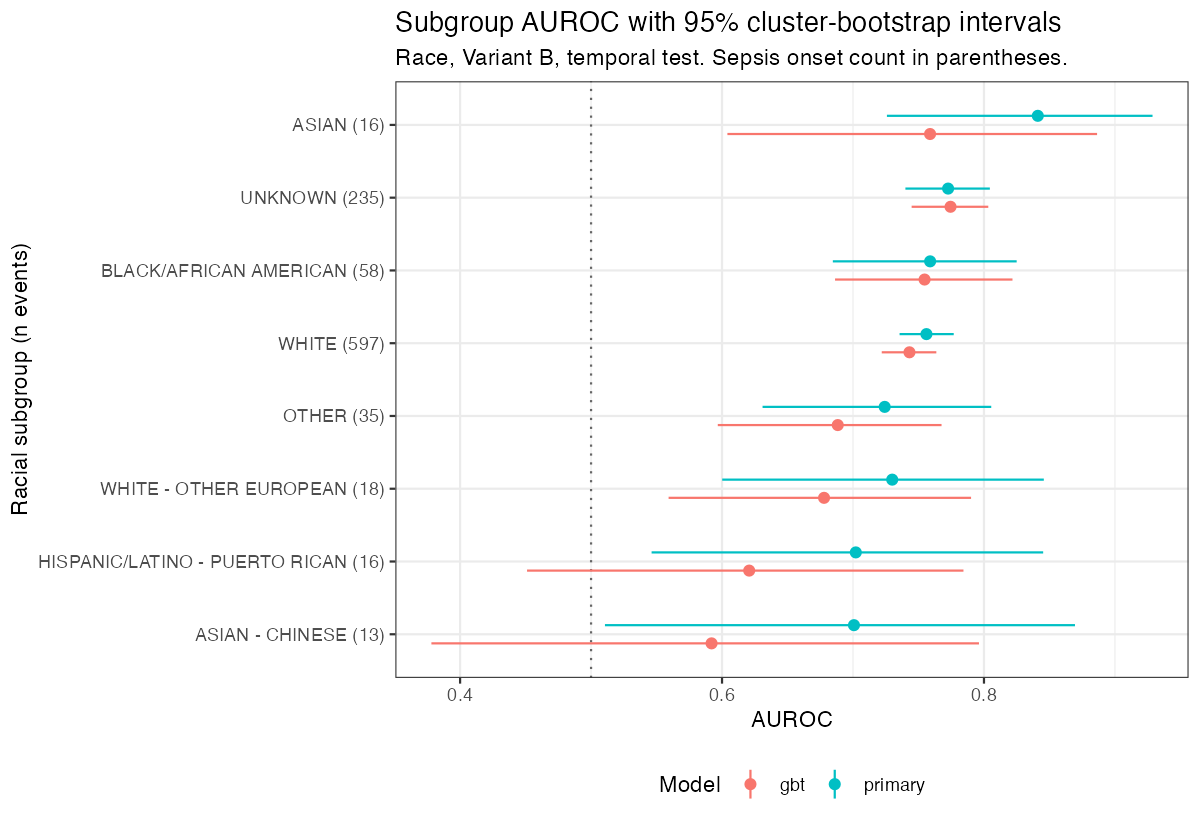
\includegraphics[width=0.92\textwidth]{images/12_subgroup_auroc_ci.png}
    \caption{AUROC by racial subgroup with 95\% stay-level cluster-bootstrap
    intervals (Variant B, temporal test); sepsis onset count in parentheses.
    Interval width is governed almost entirely by the stratum event count, and
    several intervals reach the 0.5 chance line.}
    \label{fig:auroc_by_race}
\end{figure}

\subsection{Label Sensitivity by Subgroup \texorpdfstring{[E]}{[E]}}
\label{sec:label_sens_subgroup}

\begin{table}[H]
    \centering\footnotesize
    \adjustbox{max width=\textwidth}{% GENERATED by thesis_constants.R -- do not edit
\begin{tabular}{lrcccc}
\toprule
\textbf{Racial group} & \textbf{Stays} & \textbf{A (\%)} & \textbf{B (\%)} & \textbf{C (\%)} & \textbf{Range (pp, 95\% CI)} \\
\midrule
White & 40{,}212 & 9.4 & 9.6 & 18.6 & 9.3 (8.9--9.7) \\
Unknown & 7{,}264 & 11.6 & 12.8 & 23.9 & 12.3 (11.3--13.3) \\
Black / African American & 4{,}929 & 9.3 & 9.1 & 19.0 & 9.9 (9.0--11.1) \\
Other & 2{,}254 & 8.8 & 9.8 & 17.5 & 8.7 (7.1--10.2) \\
Unable to obtain & 1{,}629 & 9.7 & 11.1 & 22.5 & 12.8 (10.7--14.9) \\
White -- Other European & 1{,}589 & 9.4 & 7.7 & 16.6 & 8.9 (7.2--10.7) \\
Asian & 799 & 10.5 & 11.5 & 21.3 & 10.8 (8.3--13.8) \\
Asian -- Chinese & 721 & 10.1 & 11.1 & 19.0 & 8.9 (6.4--11.9) \\
\bottomrule
\end{tabular}
}
    \caption{Percentage of stays labelled as septic by racial subgroup and label
    variant, with a 95\% stratified cluster-bootstrap interval on the A--C
    range. The fraction roughly doubles from Variant A to C across all groups.
    Per-variant intervals are in \texttt{12\_subgroup\_labelsens\_ci.csv}.
    \textbf{[E] exploratory.}}
    \label{tab:equity_label}
\end{table}

The fraction of patients labelled as septic changes by
\pcLabelSensRangeLo--\pcLabelSensRangeHi{} percentage points across label
variants within each racial stratum. Unlike discrimination, this contrast
survives correction, because it is a stay-level proportion computed on the full
\pcNStays{}-stay cohort rather than on the few hundred test-window onsets. No
event floor is therefore applied; the construct limitation of
Section~\ref{sec:equity_strata} still applies.

\begin{table}[H]
    \centering\footnotesize
    \adjustbox{max width=\textwidth}{% GENERATED by thesis_constants.R -- do not edit
\begin{tabular}{lrcrr}
\toprule
\textbf{Racial group} & \textbf{Stays} & \textbf{$\Delta$ range vs.\ White (pp, 95\% CI)} & \textbf{$p$} & \textbf{$q_{\text{BH}}$} \\
\midrule
Unknown & 7{,}264 & $+3.01$ ($+1.93$--$+4.06$) & 0.001 & \textbf{0.006} \\
Unable to obtain & 1{,}629 & $+3.49$ ($+1.38$--$+5.55$) & 0.002 & \textbf{0.009} \\
Black / African American & 4{,}929 & $+0.62$ ($-0.35$--$+1.87$) & 0.186 & 0.347 \\
Asian & 799 & $+1.48$ ($-1.04$--$+4.50$) & 0.249 & 0.407 \\
Other & 2{,}254 & $-0.63$ ($-2.26$--$+0.98$) & 0.425 & 0.510 \\
White -- Other European & 1{,}589 & $-0.41$ ($-2.10$--$+1.41$) & 0.635 & 0.714 \\
Asian -- Chinese & 721 & $-0.40$ ($-3.02$--$+2.61$) & 0.675 & 0.714 \\
\bottomrule
\end{tabular}
}
    \caption{Difference in label sensitivity (A--C range) against the reference
    group (White). $q_{\text{BH}}$ is adjusted over exploratory family E2, all
    18 label-sensitivity contrasts across race, language and insurance. Two
    racial contrasts survive at $q < 0.05$; across the full family,
    \pcLabelSensNSig{} do (adding Spanish-speaking patients,
    $+\pcLabelSensSpanishPp$ pp, $q = \pcLabelSensSpanishQ$, and privately
    insured patients, $\pcLabelSensPrivatePp$ pp,
    $q = \pcLabelSensPrivateQ$). \textbf{[E] exploratory.}}
    \label{tab:equity_label_contrasts}
\end{table}

\pcLabelSensNSigRace{} racial strata are significantly more label-sensitive
than the reference after false-discovery correction, and \emph{both of them are
missingness categories}: Unknown ($+\pcLabelSensUnknownPp$ pp,
$q = \pcLabelSensUnknownQ$) and Unable to obtain ($+\pcLabelSensUnablePp$ pp,
$q = \pcLabelSensUnableQ$). No stratum recording an actual demographic answer
differs from the reference. Across the full family, Spanish-speaking patients
are more label-sensitive than English-speaking patients
($+\pcLabelSensSpanishPp$ pp, $q = \pcLabelSensSpanishQ$), and privately
insured patients are \emph{less} label-sensitive than Medicare patients
($\pcLabelSensPrivatePp$ pp, $q = \pcLabelSensPrivateQ$).

The significant contrasts involve documentation-related categories and
strata of language and insurance, and may reflect differences in record
completeness; this mechanism was not tested
(Limitation~\ref{lim:subgroup}). Of the two equity analyses, only this one is
precise enough to support a claim, and reporting either without the other
would invert which conclusion the data support.

\begin{figure}[H]
    \centering
    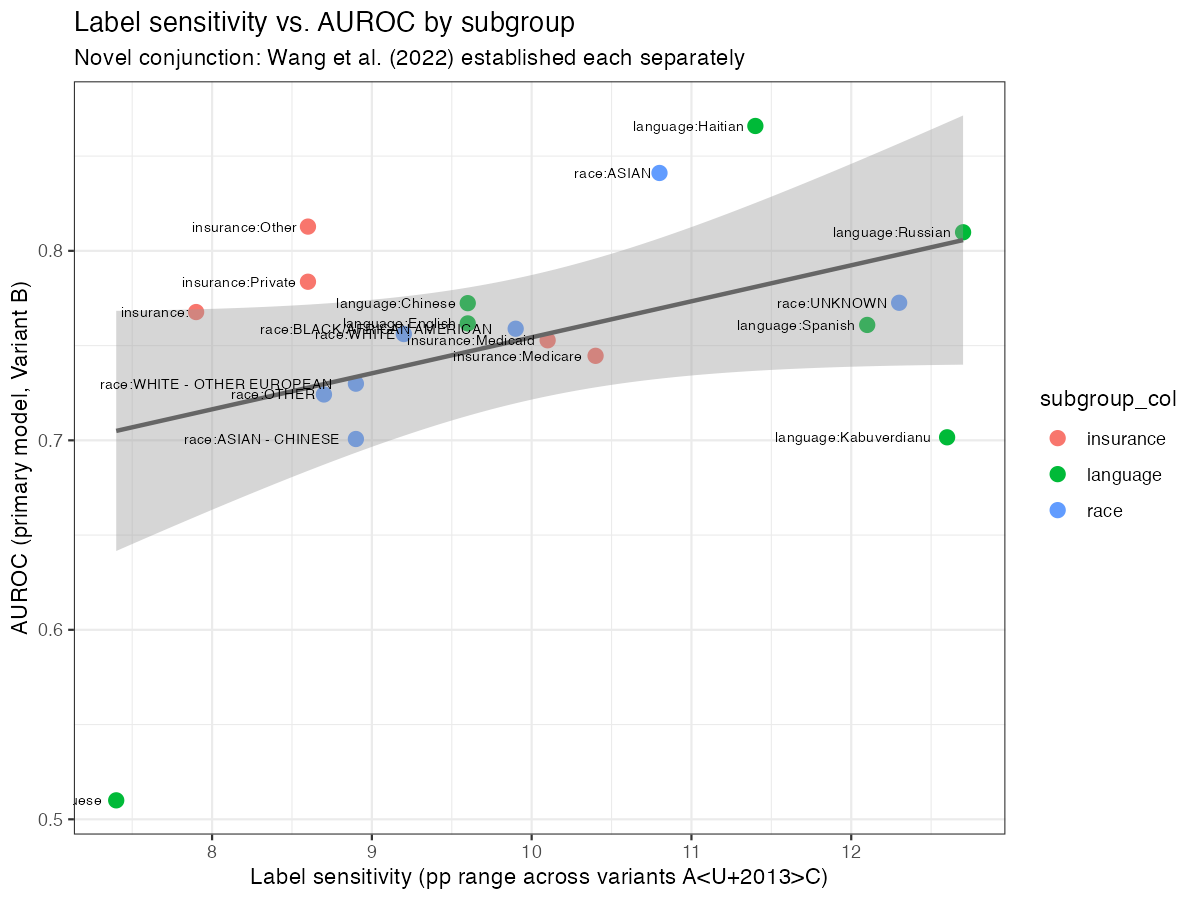
\includegraphics[width=0.85\textwidth]{images/10_label_sens_vs_auroc.png}
    \caption{Label sensitivity (fraction labelled septic) vs.\ AUROC by racial
    subgroup, across all three label variants. No association is tested, and
    the AUROC uncertainty of Figure~\ref{fig:auroc_by_race} is not shown.
    \textbf{[E] exploratory, visual only.}}
    \label{fig:label_sens_vs_auroc}
\end{figure}

%===========================================================================


\section{Variance Decomposition and Hypothesis Verdicts \texorpdfstring{[C]}{[C]}}
\label{sec:decomposition}
%===========================================================================

This section assembles the preceding estimates into the variance decomposition
and the six hypothesis verdicts. The label spread is read across the three
variants of Section~\ref{sec:internal_performance}, the model-class spread
across the model rows of the same table, the split contrast against the
random-split arm, and the transport contrast against the external estimates of
Section~\ref{sec:external_validation}. Each is an AUROC contrast with an interval
from the same stay-level cluster bootstrap.

\paragraph{Spreads as ranges.} Each spread is a \emph{range}: the largest AUROC
in a set minus the smallest. The label spread is a range over three variants and
the model-class spread over six specifications. Because a range grows with the
number of values even when the underlying quantities are identical, a range
over six is expected to exceed one over three by roughly half again, a bias
present in every bootstrap replicate (the same reason the subgroup range is not
treated as an effect size in Section~\ref{sec:equity}).

The ordering does not depend on this statistic. The model-class range spans a
structural gap rather than sampling scatter, between the two fitted
models and the four rule-based and Cox comparators, and \emph{any} single
contrast across that gap is larger than the whole label range. The narrowest of
them, GBT against the Cox model, is \pcAurocGbtB{} against \pcAurocCoxB, which
exceeds the label range by a factor of eight and involves no order statistic.
An asymmetry of about half again cannot account for \pcSpreadModelClass{}
against \pcSpreadLabel.

A variance-components partition is not used, for two reasons: the AUROCs are
computed on the same test rows, so the design supplies no suitable error term,
and \S7 of the pre-registration fixed the estimand as the \emph{spread}. The
range is reported as a descriptive summary with a bootstrap interval.

Two of the six hypotheses admit no test statistic, for reasons of design; both
still occupy a slot in the correction (Section~\ref{sec:confirmatory_verdicts}).

\subsection{The Decomposition Table}

\begin{table}[H]
    \centering\small
    \begin{tabular}{p{4.6cm}cll}
        \toprule
        \textbf{Factor (others fixed)}         & \textbf{$\Delta$AUROC} & \textbf{95\% CI} & \textbf{H} \\
        \midrule
        Model class (label B, temporal)        & \pcSpreadModelClass & \pcSpreadModelClassCiLo--\pcSpreadModelClassCiHi & n/a \\
        Label definition (primary, temporal)   & \pcSpreadLabel      & \pcSpreadLabelCiLo--\pcSpreadLabelCiHi & H1 \\
        Split method (primary, label B)        & \pcSpreadSplit      & \pcHFourCiLo--\pcHFourCiHi & H4 \\
        External transport (primary, label B)  & \pcSpreadMetric     & \pcHFiveCiLo--\pcHFiveCiHi & H5 \\
        \midrule
        GBT $-$ primary (label B, temporal)    & \pcHSixEst          & \pcHSixCiLo--\pcHSixCiHi & H6 \\
        \bottomrule
    \end{tabular}
    \caption{Variance decomposition with 95\% stay-level cluster-bootstrap
    intervals. The name is the pre-registration's (\S1) and the quantities are
    ranges, not variance components: they neither estimate nor partition a
    variance, and they are not on a common denominator, so they cannot be
    summed or expressed as shares of a total. Each row varies one factor with
    the others held fixed, over the alternatives named. The first row tests no
    hypothesis; H1 contrasts it with the label range. H6, below the rule, is the
    contrast between the two \emph{flexible} estimators alone.
    \textbf{[C] confirmatory.}}
    \label{tab:decomposition}
\end{table}

The four factors differ widely in effect. \textbf{The spread across the six
evaluated model specifications is the largest} (\pcSpreadModelClass). That set
runs from a 29-term dynamic hazard model to qSOFA and differs in features,
event handling and fitting as well as model form (Section~\ref{sec:models}), so
the claim concerns this comparison, not model architecture in general.
\textbf{External transport has the second-largest point estimate}
(\pcSpreadMetric), but its interval is the widest in the table and covers zero,
so its rank is not established. The label moves discrimination by
\pcSpreadLabel{} and the split by \pcSpreadSplit, both small, and the split's
interval covers zero. The pre-registered expectation that the four factors
would be comparable is not supported. Three qualifications apply:

\begin{itemize}
    \item Between the two \emph{flexible} estimators, fitted on identical
          covariates, the gap is \pcHSixAbsEst{}, an order of magnitude below
          the six-specification range and of the same order as the label's
          (H6; Section~\ref{sec:h6}).
    \item The label factor is small \emph{in discrimination} only. The
          variants disagree about which patients are septic
          ($\kappa = \pcKappaVsBA$, A vs B), so they define different cohorts,
          prevalences and denominators for every downstream clinical claim.
    \item The split interval [\pcHFourCiLo, \pcHFourCiHi] excludes the
          pre-registered $+0.02$ optimism threshold while covering zero. The
          transport row rests on \pcExtNEventsB{} events, and its interval
          [\pcHFiveCiLo, \pcHFiveCiHi] contains both zero and a degradation
          twice the size of the label effect.
\end{itemize}

\subsection{Corrected Confirmatory Verdicts}
\label{sec:confirmatory_verdicts}

\begin{table}[H]
    \centering\footnotesize
    \adjustbox{max width=\textwidth}{%
    \begin{tabular}{llrlr>{\raggedright\arraybackslash}p{3.6cm}}
        \toprule
        \textbf{H} & \textbf{Contrast $\theta$} & \textbf{Est.} & \textbf{95\% CI}
        & \textbf{$p_{\text{Holm}}$} & \textbf{Verdict} \\
        \midrule
        H1 & Label spread $-$ model spread   & \pcHOneEst   & \pcHOneCiLo--\pcHOneCiHi   & \pcHOnePHolm   & \pcHOneVerdict   \\
        H2 & Unstable covariates (count)     & \pcHTwoEst   & n/a                         & n/a             & Descriptive      \\
        H3 & Pre-treatment onsets (count)    & \pcPreTreatOnsetsVarB & n/a               & n/a             & Definitional     \\
        H4 & Random $-$ temporal AUROC       & \pcHFourEst  & \pcHFourCiLo--\pcHFourCiHi & \pcHFourPHolm  & \pcHFourVerdict  \\
        H5$^{\dagger}$ & Internal $-$ external AUROC$^{\dagger}$ & \pcHFiveEst  & \pcHFiveCiLo--\pcHFiveCiHi & \pcHFivePHolm  & \pcHFiveVerdict  \\
        H6 & GBT $-$ primary AUROC           & \pcHSixEst   & \pcHSixCiLo--\pcHSixCiHi   & \pcHSixPHolm   & \pcHSixVerdict   \\
        \bottomrule
    \end{tabular}}
    \caption{The confirmatory family. One-sided cluster-bootstrap tests against
    each hypothesis's pre-registered threshold ($\theta_0 = 0$ for H1, and for
    the amended AUROC transport contrast shown in H5's reserved slot; 0.02 for
    H4 and H6), Holm--Bonferroni corrected at family size $m = 6$ and
    FWER 0.05. H2 and H3 reserve a slot without contributing a p-value, which
    makes the correction on the other four stricter. H3's count is entailed by
    the onset rule (Proposition~\ref{prop:h3}). \textbf{The Verdict column
    reports the pre-registered test only}: H6's non-rejection is not evidence of
    equivalence, and its one-sided non-inferiority is read off the interval
    (Section~\ref{sec:h6}). The smallest reportable p-value is $1/(B+1)$.
    \textbf{[C] confirmatory, except $\dagger$}: H5's pre-registered estimand
    is \textbf{not evaluable}, and the row shows an \textbf{[A] amended,
    post-hoc} substitute contrast occupying its correction slot
    (Section~\ref{sec:h5}).}
    \label{tab:confirmatory}
\end{table}

H1 and H4 are not confirmed: their adjusted p-values are \pcHOnePHolm{} and
\pcHFourPHolm, and their point estimates lie on the opposite side of zero from
the one predicted. H6 is not rejected and its interval supports one-sided
non-inferiority but not two-sided equivalence. H2 is descriptive, and H3 and
H5 were not evaluable as pre-registered; the contrast substituted for H5 is
inconclusive. The following subsections give each verdict with its estimate;
the underlying results are in the sections cited.

\subsection{H1: Label Dominance (Not Confirmed)}

\begin{mdframed}[backgroundcolor=ATUOrange!20, linecolor=ATUOrange]
    \textbf{H1 [C]:} Spread in AUROC across label variants $\geq$ spread across
    model classes.

    \textbf{Point estimates:} label spread $= \pcSpreadLabel$;
    model spread $= \pcSpreadModelClass$.

    \textbf{Contrast:} $\theta = \pcHOneEst$ (95\% CI
    \pcHOneCiLo--\pcHOneCiHi), Holm-adjusted $p = \pcHOnePHolm$.
    \textbf{H1 NOT CONFIRMED; the estimate lies in the direction opposite
    to the one hypothesised.}
\end{mdframed}

Across the six evaluated specifications, model choice affected AUROC more than
the three Sepsis-3 variants did: the difference of spreads excludes zero. The
specification spread runs from rule-based scores (qSOFA \pcAurocQsofaB, SIRS
\pcAurocSirsB, NEWS2 \pcAurocNewsB) through the Cox comparator
(\pcAurocCoxB) to the two flexible estimators (primary \pcAurocPrimaryB, GBT
\pcAurocGbtB). The variants nevertheless changed cohort membership
substantially: A and B agree on only \pcPctAgreeBA\% of stays
($\kappa = \pcKappaVsBA$) despite near-identical prevalence
(Section~\ref{sec:label_anchor_results}).

\begin{figure}[H]
    \centering
    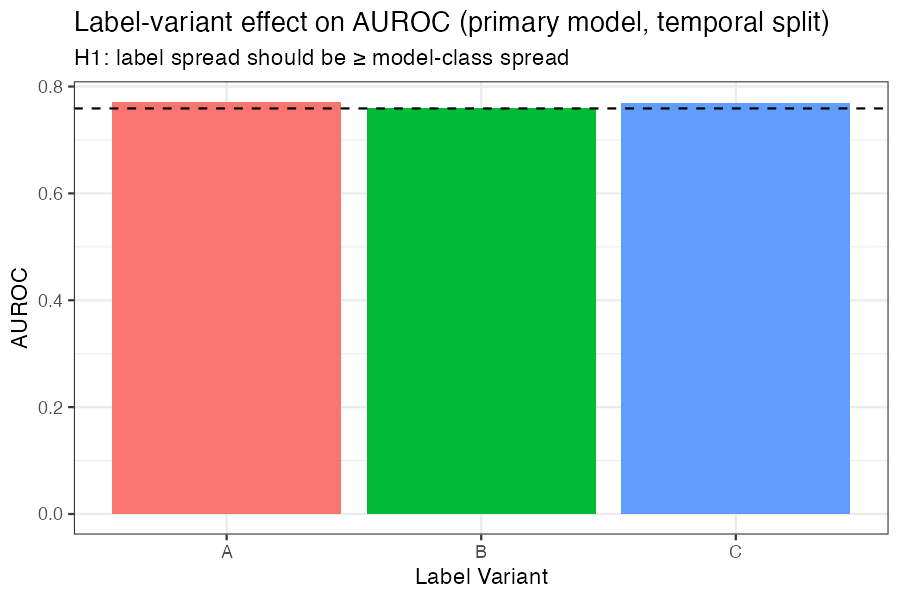
\includegraphics[width=0.85\textwidth]{images/09_label_variance_auroc.png}
    \caption{AUROC by label variant for each model (temporal split). Both
    quantities are \emph{ranges}, largest minus smallest: the range within each
    model group is the label contribution (\pcSpreadLabel, over three variants)
    and the range across groups is the spread across the six model
    specifications (\pcSpreadModelClass), larger by roughly an order of
    magnitude (Section~\ref{sec:decomposition}).}
    \label{fig:label_variance_auroc}
\end{figure}

\subsection{H2: Coefficient Instability (Met, Descriptive)}
\label{sec:h2}

\begin{mdframed}[backgroundcolor=ATUSand!30, linecolor=ATUGreen]
    \textbf{H2 [C]:} At least one feature changes sign or magnitude
    $\geq 2\times$ across label variants.

    \textbf{Result:} of the \pcHTwoNTerms{} covariates shared by all three
    variants, \pcHTwoNSign{} reverse sign, \pcHTwoNMag{} change magnitude by
    $\geq 2\times$, and \pcHTwoEst{} do at least one of the two.
    \textbf{H2's criterion is met (descriptive; no test statistic).}

    \textbf{Multiplicity:} H2 reserves a slot in the confirmatory family of six
    but contributes no p-value, which makes the Holm correction on the
    remaining hypotheses stricter rather than weaker.
\end{mdframed}

The count is the pre-registered answer, reported unmodified, and depends on the
penalised fit of Section~\ref{sec:primary_model_spec}. Because a threshold rule
on point estimates cannot separate genuine movement from imprecision, it is an
upper bound on the instability present.

\begin{table}[H]
    \centering
    \begin{tabular}{lp{8cm}}
        \toprule
        \textbf{Feature}           & \textbf{What changed}                   \\
        \midrule
        Bilirubin                  & Sign reversal across variants           \\
        Any vasopressor            & Sign reversal \emph{and} magnitude $\geq 2\times$ \\
        Platelets                  & Magnitude $\geq 2\times$                \\
        Creatinine measured        & Magnitude $\geq 2\times$                \\
        Platelets measured         & Magnitude $\geq 2\times$                \\
        WBC measured               & Magnitude $\geq 2\times$                \\
        \bottomrule
    \end{tabular}
    \caption{Features with sign reversal or magnitude instability across label
    variants. \pcHTwoNSign{} of the \pcHTwoNTerms{} shared covariates reverse
    sign and \pcHTwoEst{} are unstable on either criterion. Full per-covariate
    flags are in \texttt{12\_h2\_coefficient\_stability.csv}.}
    \label{tab:coef_instability}
\end{table}

\subsubsection{Does the instability exceed its own estimation noise? (Protocol
Amendment 7)}
\label{sec:h2_uncertainty}

Using the cluster-robust covariance (Section~\ref{sec:primary_model_spec}),
the difference between each flagged covariate's two extreme estimates is
referred to their pooled standard error (Table~\ref{tab:h2_uncertainty}).

\begin{table}[H]
    \centering\footnotesize\setlength{\tabcolsep}{4pt}
    \adjustbox{max width=\textwidth}{% GENERATED by thesis_constants.R -- do not edit
\begin{tabular}{lrrrrrrl}
\toprule
\textbf{Covariate} & \textbf{$\beta_A$} & \textbf{$\beta_B$} & \textbf{$\beta_C$} & \textbf{Max diff.} & \textbf{Pooled SE} & \textbf{Ratio} & \textbf{Kind} \\
\midrule
\texttt{wbc\_measured} & 0.0969 & 0.5374 & 0.8989 & 0.8020 & 0.0517 & 15.51 & action \\
\texttt{platelets\_measured} & -0.2563 & -0.5614 & -0.8173 & 0.5610 & 0.0529 & 10.60 & action \\
\texttt{creatinine\_measured} & 0.2877 & 0.2303 & 0.0343 & 0.2534 & 0.1024 & 2.48 & action \\
\texttt{platelets} & 0.0002 & 0.0001 & 0.0003 & 0.0002 & 0.0002 & 1.07 & physiol. \\
\texttt{vaso\_anyTRUE} & -0.0374 & 0.0271 & 0.0025 & 0.0645 & 0.0864 & 0.75 & action \\
\texttt{bilirubin\_total} & 0.0014 & -0.0016 & -0.0020 & 0.0034 & 0.0056 & 0.61 & physiol. \\
\bottomrule
\end{tabular}
}
    \caption[H2 instability against estimation noise]{Each covariate flagged by
    H2, with its coefficient under each label variant, the difference between
    the two extremes, the pooled cluster-robust standard error of those two
    estimates, and their ratio. \pcHTwoNRobust{} of the \pcHTwoNFlagged{}
    flagged covariates move by more than roughly twice their pooled standard
    error; the remaining \pcHTwoNNoise{} move by less, the largest such ratio
    being \pcHTwoZMaxNoise; no covariate falls between \pcHTwoZMaxNoise{} and
    \pcHTwoZMinRobust. ``Kind'' marks clinician action or patient physiology
    (Section~\ref{sec:h2_action}). \textbf{A diagnostic, not a test}: the fits
    share stays, and the covariance is that of the penalised estimator
    (Section~\ref{sec:primary_model_spec}).}
    \label{tab:h2_uncertainty}
\end{table}

The pre-registered count stands; the post-hoc diagnostic (Protocol
Amendment 7) is reported beside it, not in its place. The covariates whose
movement exceeds their standard errors are \pcHTwoNRobustAction{} of
\pcHTwoNRobust{} action-derived, with ratios from \pcHTwoZMinRobust{} to
\pcHTwoZMax, and all are indicators of whether a test was ordered. Both sign
reversals, bilirubin and vasopressor exposure, carry the two smallest ratios,
so no claim rests on either individually. This agrees with the by-kind split
(Section~\ref{sec:h2_action}) and the ablation (Section~\ref{sec:ablation}),
but all three are computed from the same three fitted models and are not
independent corroboration.

\subsubsection{The instability is concentrated in the action-derived features}
\label{sec:h2_action}

The covariates fall into two kinds. \textbf{Action-derived} features record
clinician behaviour (vasopressor exposure and the per-test order indicators);
\textbf{physiological} features record the patient (vital signs, laboratory
values and their rolling slopes). Table~\ref{tab:instability_by_kind} splits the
instability by kind.

\begin{table}[H]
    \centering
    \begin{tabular}{lrrr}
        \toprule
        \textbf{Feature kind} & \textbf{Covariates} & \textbf{Unstable}
        & \textbf{\% unstable} \\
        \midrule
        Action-derived & \pcHTwoNAction & \pcHTwoNUnstableAction & \pcHTwoPctUnstableAction \\
        Physiological  & \pcHTwoNPhysio & \pcHTwoNUnstablePhysio & \pcHTwoPctUnstablePhysio \\
        \bottomrule
    \end{tabular}
    \caption{H2 instability by feature kind. Action-derived covariates are a
    minority of the specification but a majority of the unstable terms.
    \textbf{[E] exploratory.}}
    \label{tab:instability_by_kind}
\end{table}

Instability is concentrated in the features that encode clinician behaviour,
which a change of label affects in a way that a heart rate is not. With
\pcHTwoNTerms{} covariates the counts are small and the difference between the
two rates is not tested. The result supports Lauritsen et al.'s
\cite{lauritsen2021framing} framing-instability concern for specific effect
estimates, not instability of the fitted model as a whole.

\subsection{H3: Treatment Leakage, Definitional and Empirical}
\label{sec:h3}

\begin{mdframed}[backgroundcolor=ATUPurple!10, linecolor=ATUPurple]
    \textbf{H3 [C]:} Restricting to pre-treatment hours reduces AUROC by
    $\geq 0.03$.

    \textbf{Definitional result:} \textbf{\pcPreTreatOnsetsVarB{} sepsis onset
    events} in \pcPreTreatPersonHoursVarB{} pre-treatment person-hours. AUROC is
    undefined, so the pre-registered contrast cannot be formed. This zero is
    \emph{proved} below (Proposition~\ref{prop:h3}) to follow from the onset
    rule used by variants A--C; it is a statement about the implementation, not
    a measurement.

    \textbf{Empirical result (Protocol Amendment 4):} relabelling the same
    stays with the standard $\min(t_{\text{susp}}, t_{\text{SOFA}})$ onset
    (Variant F) moves \pcFNMovedEarlier{} of \pcFNOnsets{} onsets earlier
    (\pcFPctMovedEarlier\%, median \pcFMedianShiftH\,h) and places
    \textbf{\pcPreTreatOnsetsVarF{} onsets before treatment}, identified at
    \pcPreTreatAurocPrimaryF{} AUROC (\pcPreTreatAurocGbtF{} GBT).
    \textbf{H3 is not evaluable as pre-registered; the definitional and
    empirical statements replace it.}

    \textbf{Multiplicity:} like H2, H3 reserves a slot in the confirmatory
    family without contributing a p-value. Variant F's contrast against B is
    exploratory (family E3).
\end{mdframed}

\paragraph{Definitional result.}
In the hours before the first antibiotic or culture there are zero onset events
for variants A--C and E. This follows from how the onset timestamp is assigned:

\begin{mdframed}[backgroundcolor=ATUSand!20, linecolor=ATUGreen]
    \begin{proposition}\label{prop:h3}
    Let $t_{\mathrm{anchor}}$ be the earlier of the first qualifying antibiotic
    order and the first culture draw of an admission, and let
    $t_{\mathrm{onset}}$ be the onset assigned by variants A, B, C or E. Then
    $t_{\mathrm{onset}} \geq t_{\mathrm{anchor}}$ for every labelled stay, so the
    window $[\,\cdot\,,\, t_{\mathrm{anchor}})$ contains no onset.
    \end{proposition}

    \emph{Proof.} Under E, $t_{\mathrm{onset}} = t_{\mathrm{susp}}$, and
    $t_{\mathrm{susp}}$ is defined as the \emph{later} element of a qualifying
    antibiotic-culture pair; both elements are at or after
    $t_{\mathrm{anchor}}$, so $t_{\mathrm{susp}} \geq t_{\mathrm{anchor}}$.
    Under A, B and C the SOFA criterion is a \emph{membership} gate: a stay is
    labelled only if the $\geq 2$-point rise occurs somewhere in the evaluation
    window, but the timestamp written is still $t_{\mathrm{susp}}$
    (Section~\ref{sec:alt_labels}). The inequality therefore carries over
    unchanged. $\square$
\end{mdframed}

\noindent The exact one-sided 95\% upper bound on the pre-treatment onset rate
in the inference tables therefore bounds a quantity the definition fixes at
zero.

\paragraph{Empirical result.}
Under the standard $\min(t_{\text{susp}}, t_{\text{SOFA}})$ onset
(Equation~\ref{eq:early_onset}), an onset precedes the anchor whenever the SOFA
rise is detected before the clinician acts, and Proposition~\ref{prop:h3} does
not apply. Variant F, with the same septic stays as Variant B, records
\pcPreTreatOnsetsVarF{} pre-treatment onsets in the temporal test set,
identified at \pcPreTreatAurocPrimaryF{} AUROC
(Section~\ref{sec:pretreatment_label}). The conjunction-timing rule of the
pre-registered variants is therefore what prevents pre-treatment onsets from
being recorded; Section~\ref{sec:discussion_core} interprets this result.

\subsection{H4: Split Optimism (Not Confirmed)}
\label{sec:h4_discussion}

\begin{mdframed}[backgroundcolor=ATUOrange!20, linecolor=ATUOrange]
    \textbf{H4 [C]:} Temporal-split AUROC is at least 0.02 lower than
    random-split AUROC.

    \textbf{Result:} primary model, random AUROC \pcAurocRandomPrimaryB{}
    against temporal \pcAurocPrimaryB. Difference $= \pcHFourEst$ (95\% CI
    \pcHFourCiLo--\pcHFourCiHi): the temporal split is the \emph{higher} of
    the two. Test against the pre-registered threshold $\theta_0 = 0.02$:
    Holm-adjusted $p = \pcHFourPHolm$. \textbf{H4 NOT CONFIRMED.}
\end{mdframed}

\begin{table}[H]
    \centering
    \begin{tabular}{llrr}
        \toprule
        \textbf{Model} & \textbf{Temporal} & \textbf{Random} & \textbf{Random $-$ temporal} \\
        \midrule
        Primary & \pcAurocPrimaryB & \pcAurocRandomPrimaryB & \pcSplitDeltaPrimaryB \\
        GBT     & \pcAurocGbtB     & \pcAurocRandomGbtB     & \pcSplitDeltaGbtB \\
        Cox     & \pcAurocCoxB     & \pcAurocRandomCoxB     & \pcSplitDeltaCoxB \\
        NEWS2   & \pcAurocNewsB    & \pcAurocRandomNewsB    & \pcSplitDeltaNewsB \\
        \bottomrule
    \end{tabular}
    \caption{Temporal vs.\ random split comparison (Variant B, AUROC). Every
    model scores lower on the random split.}
    \label{tab:split_optimism}
\end{table}

The interval includes zero and excludes $+0.02$, and all four models fitted
under both splits score lower on the random split, by \pcSplitDeltaMinAbs{} to
\pcSplitDeltaMaxAbs. The temporal test set is the 2017--2019 cohort whereas the
random test set spans all years, so the contrast also confounds split design
with cohort composition, and the random split cannot be assumed to be the more
permissive design (Section~\ref{sec:limitations}).

\subsection{H5: Metric Divergence (Not Evaluable as Pre-Registered)}
\label{sec:h5}

\begin{mdframed}[backgroundcolor=ATUOrange!20, linecolor=ATUOrange]
    \textbf{H5 [C]:} Utility Score declines proportionally more than AUROC from
    internal to external validation.

    \textbf{Testable arm:} AUROC degradation internal $\to$ external (primary,
    Variant B) $= \pcHFiveEst$ (95\% CI \pcHFiveCiLo--\pcHFiveCiHi); internal
    \pcAurocPrimaryB, eICU-CRD \pcExtAurocPrimaryB{} on \pcExtNEventsB{}
    external events. Holm-adjusted $p = \pcHFivePHolm$.
    \textbf{The point estimate falls, but the interval does not exclude no
    change.}

    \textbf{Non-testable arm:} the internal Utility Score is
    \pcUtilityPrimaryB{} at the default cut-off and \pcUtilityMaxPrimaryB{} at
    its best threshold, so a proportional decline cannot be formed.
    \textbf{H5 AS PRE-REGISTERED IS NOT EVALUABLE; the substituted AUROC
    contrast is not supported.}
\end{mdframed}

H5's proportional contrast requires a non-zero internal Utility Score, and the
internal score under the primary label is \pcUtilityPrimaryB{} at the default
cut-off and \pcUtilityMaxPrimaryB{} at its best threshold, so the contrast
cannot be formed. Its slot is occupied by the AUROC limb alone (\S13.6 of
\texttt{00\_preregistration.md}), to which the Holm-adjusted \pcHFivePHolm{}
applies. That contrast, \pcHFiveEst{}, is in the predicted direction and about
three-quarters of the 0.085 anticipated from Moor et al.\
\cite{moor2023review}, but its interval is consistent with both no loss and a
loss twice as large, because it rests on \pcExtNEventsB{} external events
(Section~\ref{sec:external_coverage}). The Narrow label loses most and the
Liberal least, and the antibiotic-only arm, a different target on
\pcExtAbxNEventsB{} events, shows a degradation of the same sign
(\pcAurocPrimaryB{} to \pcExtAbxAurocPrimaryB); neither observation is a test.

\subsection{H6: Model-Class Null (Not Rejected; One-Sided Non-Inferiority)}
\label{sec:h6}

\begin{mdframed}[backgroundcolor=ATUSand!30, linecolor=ATUGreen]
    \textbf{H6 [C]:} $|\Delta_\text{AUROC}(\text{GBT} - \text{primary})| \leq 0.02$.

    \textbf{Result:} $\Delta = \pcHSixEst$ (GBT \pcAurocGbtB, primary
    \pcAurocPrimaryB), 95\% CI \pcHSixCiLo--\pcHSixCiHi. The \emph{upper} limit
    lies inside the bound $\theta_0 = 0.02$; the lower limit does not.
    \textbf{H6 NOT REJECTED. The interval supports one-sided non-inferiority
    of the primary model (GBT is not better by more than the margin), not
    two-sided equivalence.}
\end{mdframed}

Both models are scored on the same person-hours, so the contrast is paired,
and the primary model is also ahead under the other two labels
(Table~\ref{tab:internal_results}). The pre-registered form (\S7) places
equivalence in the \emph{null}, $H_0\colon |\theta| \leq 0.02$; \textbf{this
is not the two one-sided tests (TOST) procedure}, and failure to reject the
interval null is not evidence of equivalence. Protocol Amendment 10 tests both
boundaries: at $\theta = +0.02$ $p = \pcHSixPLimbUpper$, and at
$\theta = -0.02$ $p = \pcHSixPLimbLower$. Neither boundary is cleared, so H6 is
not rejected.

The conclusion rests on the interval. Its upper limit, \pcHSixCiHi, lies below
$+0.02$, so GBT is not supported as outperforming the primary model by the
pre-registered margin: a one-sided non-inferiority conclusion, the only form
claimed. Its lower limit, \pcHSixCiLo, falls outside $-0.02$, so two-sided
equivalence is not established. The interval lies entirely below zero, so the
primary model is ahead by \pcHSixEst{} AUROC, of the same order as the label
spread. The results therefore do not support choosing GBT over the primary
model on discrimination. A caution on the comparator's fitting procedure is
stated in Section~\ref{sec:limitations}.

The AUROC difference is not accompanied by a clinically meaningful utility
advantage for either model: at each model's best threshold GBT is marginally
ahead, \pcUtilityMaxGbtB{} against \pcUtilityMaxPrimaryB, and both maxima lie
a few per cent above the no-alert strategy.

\begin{figure}[H]
    \centering
    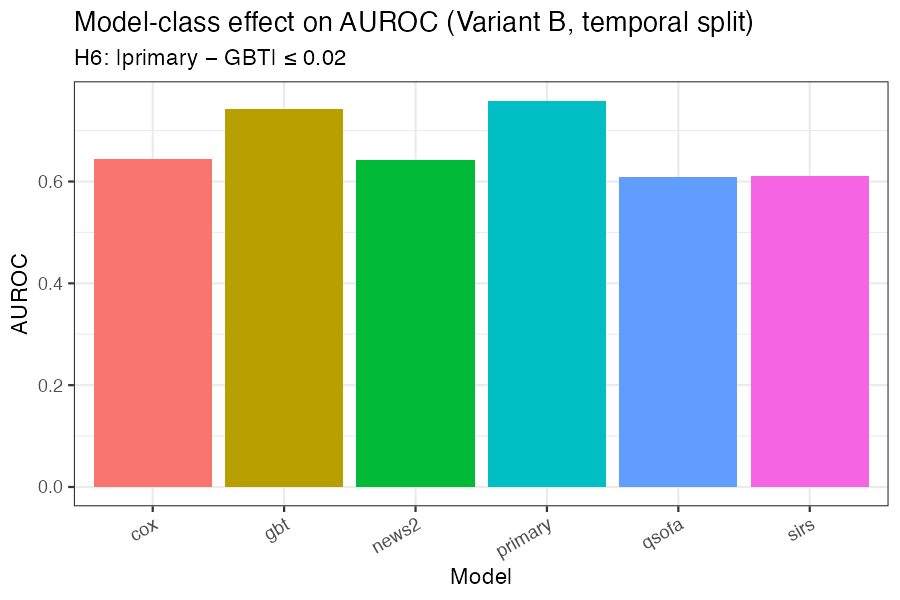
\includegraphics[width=0.85\textwidth]{images/09_model_class_auroc.png}
    \caption{AUROC by model class (Variant B, temporal split). The two flexible
    estimators are close to one another and clearly ahead of the rule-based
    scores and the Cox comparator; on the paired contrast the primary model
    leads GBT by \pcHSixAbsEst{} (Section~\ref{sec:h6}).}
    \label{fig:model_class_auroc}
\end{figure}

